\clearemptydoublepage
\acresetall
\chapter{Machine Learning and Classification Principles}
\label{chp:chapter2}
\section{Introduction} \label{sec:chp2-sec1}
Machine learning is refers to a set of methods that can automatically detect patterns in data and use them in decision making and future data prediction~\cite{murphy2012machine}. 
Machine learning techniques are usually divided into two groups: descriptive (or unsupervised) and predictive (or supervised) learning.

Unsupervised learning intends to find ``interesting structures'' in a given data without any additional information about the expected output. 
These techniques formulate their problems as unconditional density estimation and multivariate probability models. 
Clustering approaches and dimension reduction methods, \acf{pca}, and graph structures are two examples of unsupervised learning.   

Supervised learning intends to find a mapping $f(.)$ which relates a set of inputs $x$ to a set of outputs $y$. 
The learning is comprehended using a set of $N$ samples and their labels $D = \{(x_{i}, y_{i})\}^{N}_{i = 1}$, called the training set.
The samples $x_{i}$ can vary from 2-D points in Cartesian coordinates to more complex forms such as images, sentences, time series, graphs, etc.
Similarly, the labels $y_{i}$ can be represented by any structure, however, in most methods they are considered to be either categorical or numerical. 
Supervised learning is known as a classification problem when $y_{i}$ is categorical; and when $y_{i}$ is a real value the problem is referred to as regression~\cite{murphy2012machine}. 

In this research, we are interested in supervised learning, and the classification problem in particular. 
Classification aims to map a set of inputs to a set of outputs, where the outputs are divided into different classes, $y \in \{1,...,C\}$.
%{\color{green}As previously mentioned classification aims to maps a set of input $x$ to a set of output $y$, where $y \in \{1,...,C\}$ and C is the number of classes.} 
If $C = 2$, it is a binary classification problem, while $C > 2$ makes it a multiclass classification. 
This project aims to separate melanoma from all other pigmented skin lesions, thus addressing a binary classification problem. 

Classification has numerous applications in real life.
Some of the most common and challenging areas include email spam filtering, data mining, face detection and recognition, document classification, and the problem of cancer detection among others.
In order to solve a classification problem, a framework consisting of several generic steps is required.
Figure~\ref{fig:GCF} shows such a general framework whose steps are described in the following sections of this chapter. 
Due to the broad studies of \ac{cad} systems of melanoma using dermoscopic images, in comparison to Stokes polarimetry, each step covers the state of the art related to conventional dermoscopic approaches.

%\tikzstyle{block} = [rectangle, draw, fill= blue!20,
%   text width=7em, text centered, rounded corners, minimum height=4em , minimum width = 7em]
%\tikzstyle{line} = [draw, -latex']
%\tikzstyle{block2} = [rectangle, draw, fill=gray!20,
%    text width=7em, text centered, rounded corners, minimum height=4em, minimum width = 7em]
%\tikzstyle{block3} = [rectangle, draw, fill=blue!40,
%    text width=7em, text centered, rounded corners, minimum height=3em , minimum width = 7em]
%\def\blockdist{1}
%\def\edgedist{1.5}
    \tikzstyle{block} = [rectangle, draw, fill=blue!30,text = black,
    text width=6em, text centered, rounded corners, minimum height=4em , minimum width = 7em]
    \tikzstyle{line}=[draw, -latex']
	\tikzstyle{block2} = [rectangle, draw, fill=white!20,
    text width=6em, text centered, rounded corners, minimum height=4em, minimum width = 7em]
    \tikzstyle{block3} = [rectangle, draw, fill=blue!30, text = black,
    text width=7em, text centered, rounded corners, minimum height=4em , minimum width = 7em]
\def\blockdist{1}
\def\edgedist{1.5}
\begin{figure}
\centering   
\begin{tikzpicture}[node distance = 1cm,scale=0.8, every node/.style={scale=0.8}]
    % Place nodes
	\node[block2] (input) {Input Data}; 
	\node[block, right of= input , node distance = 3cm](pp){Pre-processing};
	\node[block, right of = pp, node distance = 3 cm](fe){Feature extraction}; 
	\node[block, right of = fe, node distance = 3 cm](fr){Feature representation}; 
	\node[block, right of = fr, node distance = 3 cm](db){Data balancing}; 
	\node[block, right of = db, node distance = 3 cm](clas){Classification}; 
	
	% --- The arrows 
	
	%\path(pp)+(-0.8,0) node (n) {};
	\path [line] (input) -- (pp);
    \path [line] (pp) -- (fe);
    \path [line] (fe) -- (fr);
    \path [line] (fr) -- (db);
    \path [line] (db) -- (clas);
   

\end{tikzpicture}
\caption[General classification framework]{General classification framework.}
\label{fig:GCF}
\end{figure}
 

\section{Preprocessing} \label{sec:chp2-sec2}
Data preprocessing is an essential and important step in machine learning. 
This step ensures the quality of the data before further analysis and serves to compensate their imperfections. 
Thus, preprocessing acts as a foundation and assures precision in the developed framework.
In our research, samples are represented by images that must be preprocessed prior to further analysis to account for artifacts and variations in the images acquisition.
Moreover, despite that some studies treated image segmentation as an individual step~\cite{barata2013towards,capdehourat2009pigmented,celebi2007methodological}, we consider it as part of the preprocessing step, alongside image enhancement, denoising, and hair removal.
%Image enhancement, hair removal and segmentation are explained in the following as part of the preprocessing step.

%However in some studies it is treated as individual step.
%Image enhancement, hair removal and segmentation are explained in the following as part of preprocessing step.


\subsection{Image enhancement}\label{subsec:pp-enh}
Image enhancement is a set of adjustment processes on an image that make it more suitable for a specific application. 
Histogram equalization, gamma transformation, contrast and edge enhancement, illumination correction, white and color balancing, color calibration, as well as denoising belong to image enhancement techniques. 
%Contrast and edge enhancement or smoothing can be applied in frequency or spatial domain. 
In the field of skin imaging, among the aforementioned techniques, median filtering is mostly used to suppress noise, bright spots, reflections and small pores on the skin ~\cite{Chiem2007,Berenguer2009,Ruiz2011}. 
While this technique removes certain noise and artifacts, it also smooths the texture and border of the lesion, which is undesirable. 
%Probably, from lesion diagnosis point of view, the most important enhancement which can be applied is color calibration and correction. 
From the lesions diagnosis point of view, perhaps the most important enhancement concerns color calibration and correction. 
This operation aims to recover real colors of an image, allowing for more reliable use of color information in manual and automatic diagnosis~\cite{korotkov2012computerized}. 
The need for color correction while using the \acf{jpeg} format as opposed to RAW images was recently highlighted in~\cite{Quintana2011,Wighton2011a,celebiautomated}.
Figure~\ref{fig:Quintana1} shows \acf{awb}, \acf{cwb} and \ac{jpeg} color calibrated dermoscopic images acquired with two polarized cameras, while 
Fig.~\ref{fig:Quintana2} demonstrates the importance of calibrating RAW data in comparison with \ac{jpeg} dermoscopic images.



\begin{figure}
\centering
\subfloat[\ac{awb}]{
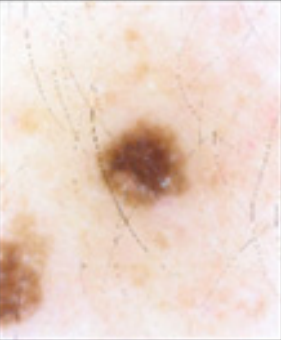
\includegraphics[height = 0.18\textheight, width= 0.16\textwidth]{Chapter2/Figures/quintana-awb_ex1.png}}\
\subfloat[\ac{cwb}]{
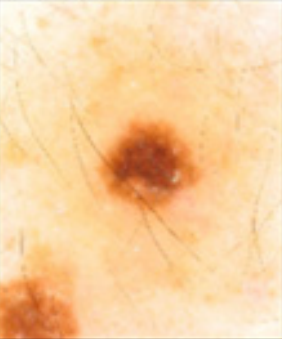
\includegraphics[height = 0.18\textheight, width= 0.16\textwidth]{Chapter2/Figures/quintana-cwb_ex1.png}}\
\subfloat[calibrated]{
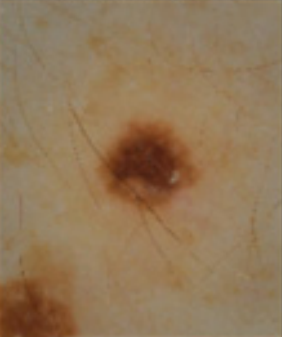
\includegraphics[height = 0.18\textheight, width= 0.16\textwidth]{Chapter2/Figures/quintana-calibrated_ex1.png}}\\
\subfloat[\ac{awb}]{
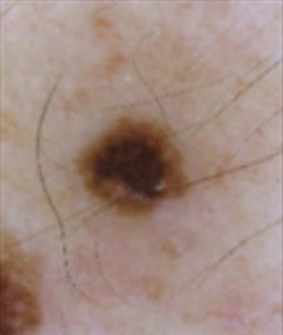
\includegraphics[height = 0.18\textheight, width= 0.16\textwidth]{Chapter2/Figures/quintana-awb_ex2.png}}\
\subfloat[\ac{cwb}]{
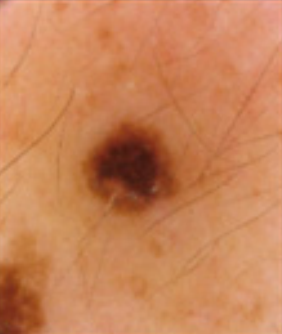
\includegraphics[height = 0.18\textheight, width= 0.16\textwidth]{Chapter2/Figures/quintana-cwb_ex2.png}}\
\subfloat[calibrated]{
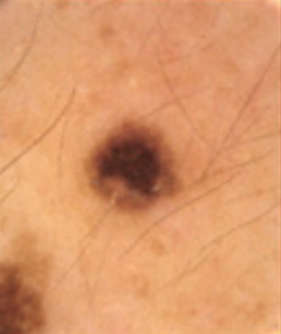
\includegraphics[height = 0.18\textheight, width= 0.16\textwidth]{Chapter2/Figures/quintana-calibrated_ex2.png}}
\caption[Color variations of dermoscopic images]{Variation in color depending on \Ac{awb}, \Ac{cwb} and \ac{jpeg} color calibration between images taken from two different dermoscopes. Images in the first row were taken with a Canon-A640 polarized dermoscope and the images in the second row were acquired with a Canon-G7 polarized dermoscope. Images are taken from~\cite{Quintana2011}.}
\label{fig:Quintana1}
\end{figure} 
 
\begin{figure}
\centering
\subfloat[\ac{cwb}]{
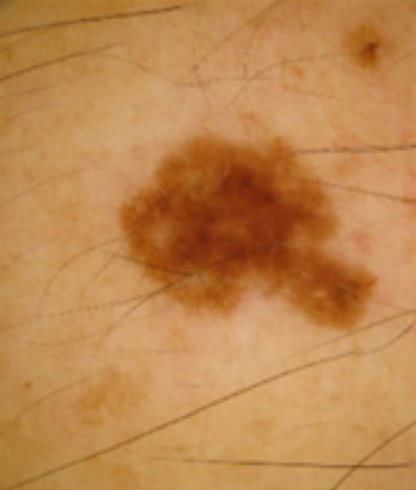
\includegraphics[height = 0.2\textheight, width= 0.19\textwidth]{Chapter2/Figures/quintana_cwb_ex3.png}}\
\subfloat[Calibrated-\ac{jpeg}]{
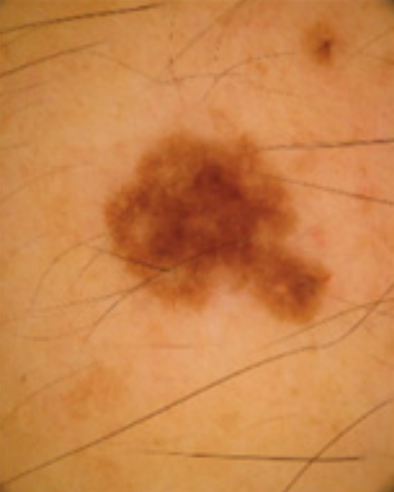
\includegraphics[height = 0.2\textheight, width= 0.19\textwidth]{Chapter2/Figures/quintana_JPEGCal_ex3.png}}\
\subfloat[Calibrated-RAW]{
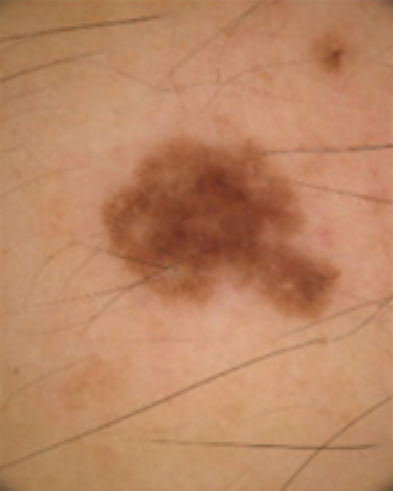
\includegraphics[height = 0.2\textheight, width= 0.19\textwidth]{Chapter2/Figures/quintana_RAWCal_ex3.png}}\\
\subfloat[\ac{cwb}]{
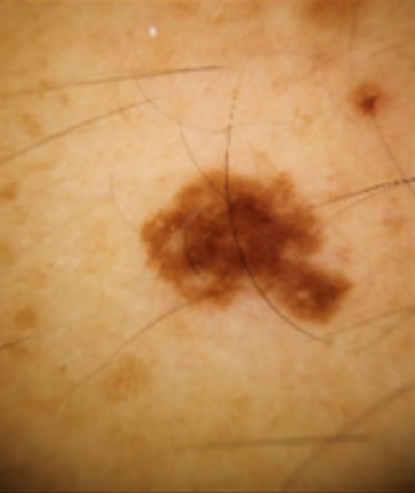
\includegraphics[height = 0.2\textheight, width= 0.19\textwidth]{Chapter2/Figures/quintana_cwb_ex4.png}}\
\subfloat[Calibrated-\ac{jpeg}]{
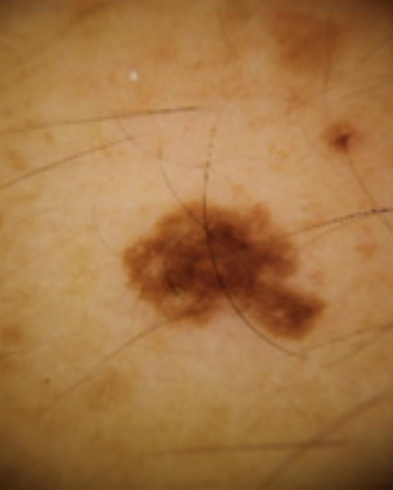
\includegraphics[height = 0.2\textheight, width= 0.19\textwidth]{Chapter2/Figures/quintana_JPEGCal_ex4.png}}
\subfloat[Calibrated-RAW]{
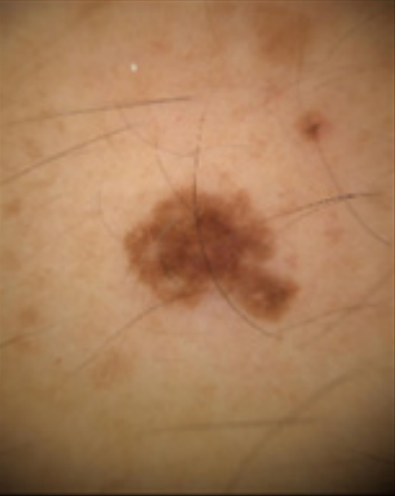
\includegraphics[height = 0.2\textheight, width= 0.19\textwidth]{Chapter2/Figures/quintana_RAWCal_ex4.png}}
\caption[Color variations between calibrated \ac{jpeg} and RAW images]{Variations in color between \Ac{cwb}, calibrated \ac{jpeg} and calibrated RAW images obtained with 2 different polarized dermoscopes. Images in the first row were acquired with Canon-G9 polarized dermoscope, while those in the second row were acquired with a Canon-5D polarized dermoscope. Images were taken from~\cite{Quintana2011}.}
\label{fig:Quintana2}
\end{figure}

\subsection{Artifacts removal} \label{subsec:artifactsremov}
Artifacts removal refers to noise removal in most image processing applications. 
However, in the field of skin imaging, it generally refers to elimination of hair, skin pores, ruler marks, air bubbles and specular reflections (see Fig.\ref{fig:artifacts}).
\begin{figure}
\centering
\subfloat[]{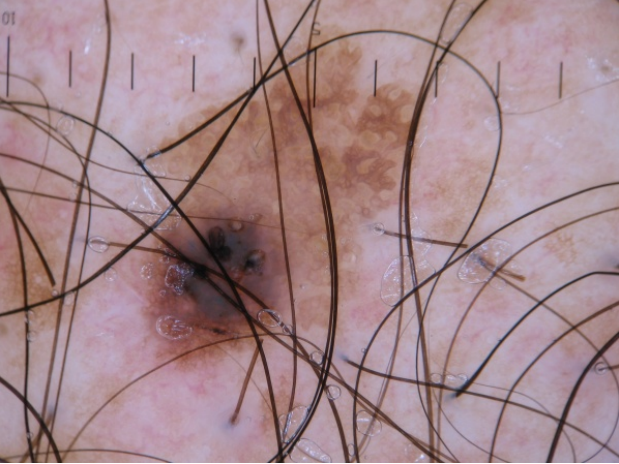
\includegraphics[height = 0.2\textheight, width= 0.3\textwidth]{Chapter2/Figures/artifacts-Hair-airbubble-Ruler.png}}\
\subfloat[]{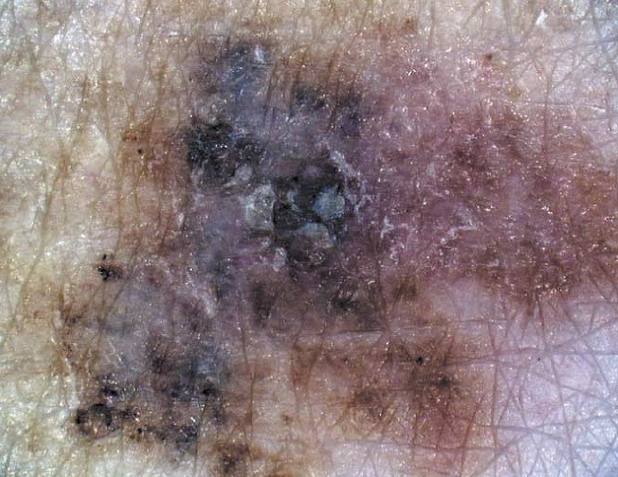
\includegraphics[height = 0.2\textheight, width= 0.3\textwidth]{Chapter2/Figures/artifacts-SpecularReflection.png}}
\caption[Artifacts in dermoscopic images]{Artifacts in dermoscopic images: (a) hair, air bubbles and ruler marks, (b) specular reflection. The images are taken from Zhou~et al.\,\cite{Zhou2008a} and Gutenev~et al.\,\cite{Gutenev2001}, respectively.}
\label{fig:artifacts}
\end{figure}
Among these operations, hair removal is the most common and necessary step.  
If a lesion is occluded by hairs, their removal is essential to achieve correct segmentation and texture analysis.
To avoid digital hair removal, the patients are usually asked to shave before image acquisition.

A hair removal algorithm commonly consists of two steps: hair detection and hair restoration (or ``inpainting'')~\cite{korotkov2012computerized}.
Inpainting fills the image space previously occupied by hairs with estimated intensity/color values. 
Considering that original colors and borders of a lesion play an essential role in lesion diagnosis, intensity estimation of missing pixels is crucial and the best inpainting method should be applied. 
\begin{figure}
\hspace*{\fill}
\subfloat[]{
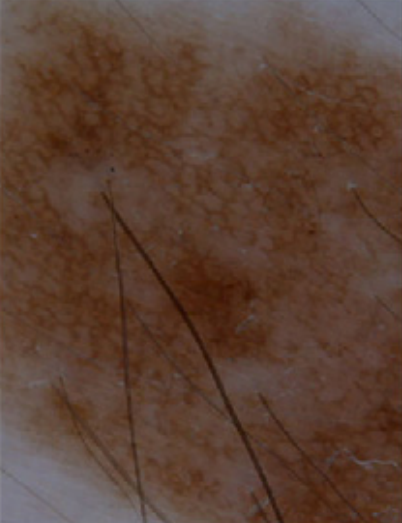
\includegraphics[height= 0.33\textheight, width= 0.3\textwidth]{Chapter2/Figures/Abas-comparison-original.png}}\hfill
\subfloat[]{
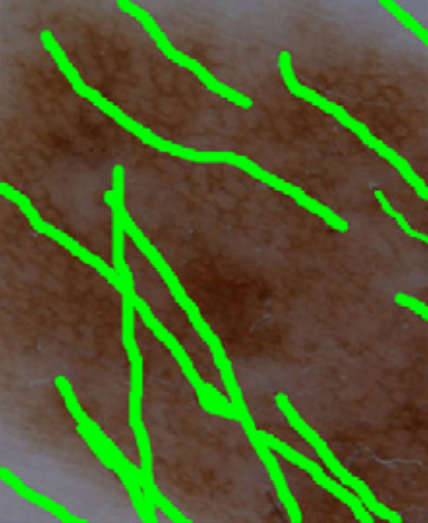
\includegraphics[height= 0.33\textheight, width= 0.3\textwidth]{Chapter2/Figures/Abas-comparison-mask.png}}\hfill
\subfloat[]{
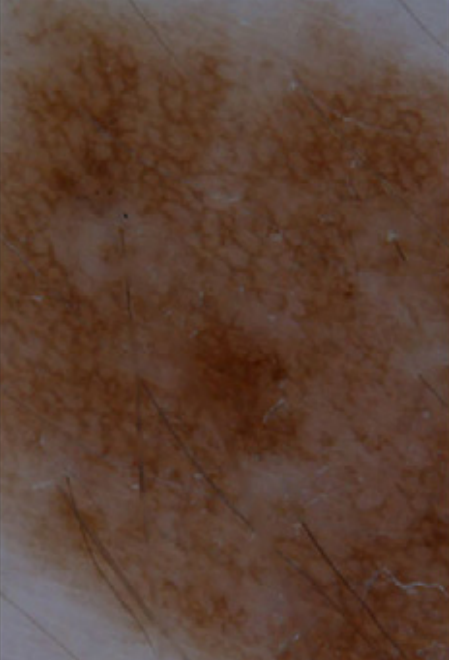
\includegraphics[height= 0.33\textheight, width= 0.3\textwidth]{Chapter2/Figures/Abas-comparison-dullruze.png}}
\hspace*{\fill}\\
\hspace*{\fill}
\subfloat[]{
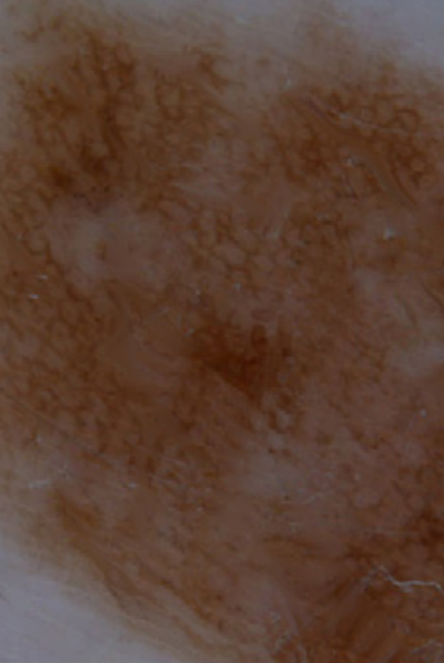
\includegraphics[height= 0.33\textheight, width= 0.3\textwidth]{Chapter2/Figures/Abas-comparison-d.png}}\hfill
\subfloat[]{
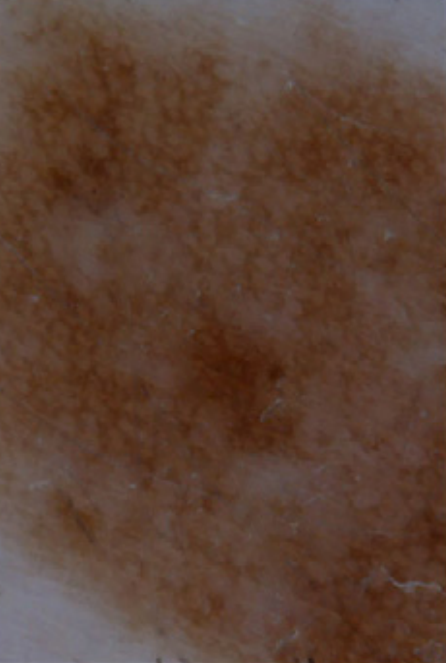
\includegraphics[height= 0.33\textheight, width= 0.3\textwidth]{Chapter2/Figures/Abas-comparison-e.png}}\hfill
\subfloat[]{
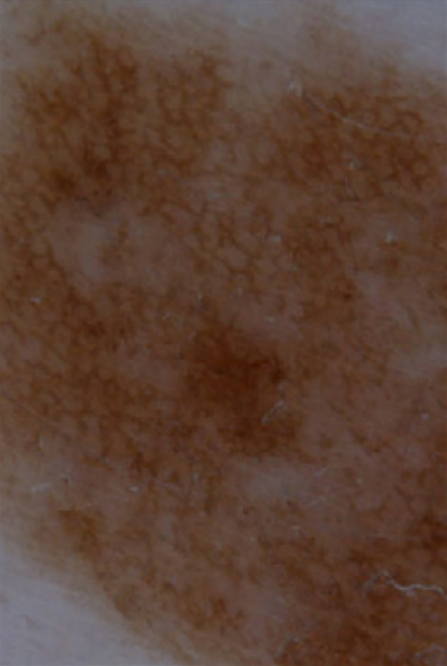
\includegraphics[height= 0.33\textheight, width= 0.3\textwidth]{Chapter2/Figures/Abas-comparison-fastmarching.png}}
\hspace*{\fill}
\caption[Comparison of inpainting methods]{Comparison of state of the art inpainting methods for hair removal algorithms. (a) Original image, (b) Highlighted hair mask, (c) DullRazor, (d) \ac{pde} non-linear inpainting, (e) exemplar-based inpainting, and (f) fast marching inpainting. The images are taken from \cite{Abbas2011a}.}
\label{fig:Abas-Comparison-repair}
\end{figure}
Lee~et al.\,\cite{Lee1997} proposed the first hair removal algorithm, DullRazor\textsuperscript{\textregistered}, for dermoscopic images. 
Kiani and Sharafat~\cite{Kiani2011} improved this algorithm to remove light-colored hairs as well as dark. 

Considering hair detection as a pixel classification problem, supervised learning was also applied in some studies~\cite{Debeir1999,Wighton2011}.
A recent survey on the topic was published by Abbas~et al.\,\cite{Abbas2011a}, where he reviewed the existing methods and proposed a broad classification based on the inpainting algorithms employed~\cite{korotkov2012computerized}: linear interpolation techniques~\cite{Lee1997,Fleming1998,Schmid-Saugeon2003,Nguyen2010}, inpainting by nonlinear \ac{pde}-based diffusion algorithms~\cite{Chung2000,Barcelos2009,Xie2009,Abbas2010a} and exemplar-based methods~\cite{Zhou2008a,Wighton2008,Abbas2010}. 
The authors~\cite{Abbas2011a,Abbas2012b} also proposed their own inpainting method based on fast marching inpainting. 
Figure~\ref{fig:Abas-Comparison-repair} shows an example demonstrating the results they achieved using different inpainting techniques.

\subsection{Image segmentation} \label{subsec:imgseg}
Image segmentation aims to decompose the image into meaningful parts with respect to a unique application. 
This technique uses image information such as grey level, texture, and color to divide the image into non-overlapping parts. 
Based on the information used, segmentation techniques are divided into four main groups: region-based, edge-based, clustering-based, and texture-based methods. 
Segmentation is also achievable via supervised learning. 

In automatic detection of melanoma, border delineation of the lesions is achieved by segmentation.
This is a challenging task due to variations in color, size, shape and texture of \ac{psls}, as well as occlusions and artifacts. 
In addition to the aforementioned challenges, segmentation algorithms face a problem of ground truth.  
%Moreover, due to difference of opinion among dermatologists and the fact that they do not require to delineate the lesion borders for their diagnosis~\cite{Day2001}, there is a ground truth problem.
It is very difficult to have a unique ground truth because dermatologists do not need to delineate lesion borders to make a diagnosis, and moreover, their individual delineations may vary significantly (see Fig.~\ref{fig:GTproblem}). 
So, normally the ground truth is generated as a fusion of different delineations done by experts. 
\begin{figure}
\centering
\subfloat[]{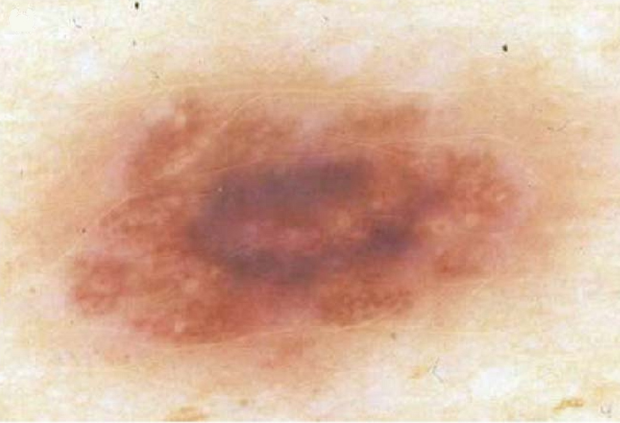
\includegraphics[height = 0.2\textheight, width= 0.3\textwidth]{Chapter2/Figures/Iyatomi-GT-original.png}}\	
\subfloat[]{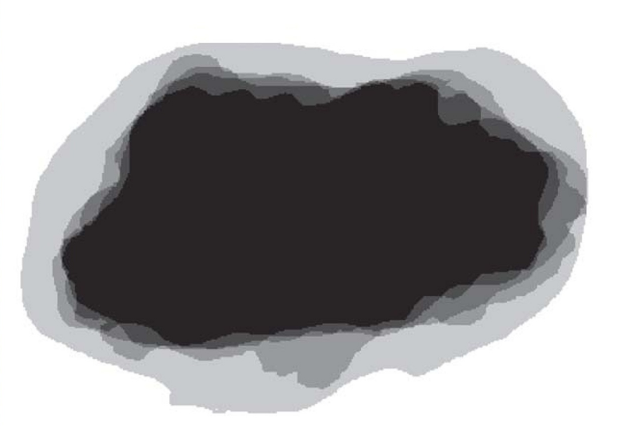
\includegraphics[height = 0.2\textheight, width= 0.3\textwidth]{Chapter2/Figures/Iyatomi-GT-5D.png}}
\caption[Lesion delineation variations]{Example of manual delineation of clark nevus by 5 dermatologists. (a) Dermoscopy image, (b) Delineation by 5 dermatologists. Images are taken from Iyatomi~et al.\,\cite{Iyatomi2006}.}
\label{fig:GTproblem}
\end{figure}
Despite these challenges, numerous methods were proposed by the research community to tackle this problem.
Good comparisons of segmentation methods for dermoscopy images were published by Silveira~et al.\,\cite{silveira2009comparison}, Celebi ~et al.\,\cite{Celebi2009a}, and Ferreira~et al.\,\cite{ferreira2013wide}.  %Korotkov~et al.\,\cite{korotkov2012computerized}
The proposed methods can be categorized based on different criteria, for instance, technical properties, level of automation or their complexity.
A review of all the proposed methods is beyond the scope of this research. 
However, an overview of available reviews and certain approaches is presented in the following.

Thresholding was one of the first approaches applied to lesion segmentation.
This technique was applied in a single color channel at first~\cite{Gutkowicz-Krusin1997,Fleming1998} and then evolved to more sophisticated approaches such as iterative thresholding~\cite{Rajab2004}, type-2 fuzzy logic based thresholding~\cite{Yuksel2009}, fusion of thresholds~\cite{Celebi2009c,Celebi2010, Celebi2013}, hybrid~\cite{Garnavi2011}, local entropy~\cite{Abbas2013a} and color histogram thresholding~\cite{Peruch2013}.

Among the many segmentation approaches developed, a variety of methods were employed such as clustering~\cite{Schmid1999b, Zhou2009, Mete2011, Liu2012}, active contours~\cite{Yuan2009, Zhou2011a,Erkol2005}, supervised learning~\cite{Debeir1999, Wighton2011, Wighton2011b, Zortea2011}, and dynamic programming~\cite{Abbas2012}, just to name a few~\cite{korotkov2012computerized}.

It is clear that without a common dataset, a comparison of the proposed methods cannot be made. 
In this regard, some studies surveyed a comparison of several methods on their own datasets~\cite{Hance1996,Silveira2009,Celebi2007,Celebi2008a,ferreira2013wide}.

Six segmentation methods (split-and-merge, center split, multiresolution, fuzzy c-mean, PCT/median cut and adaptive thresholding) were compared in~\cite{Hance1996}, where the two latter approaches outperformed the others~\cite{korotkov2012computerized}.
Silveira~et al.\,\cite{Silveira2009} also made a comparison of 6 different methods including the level set, adaptive thresholding, expectation-maximization level set, fuzzy-based split-and-merge, adaptive snakes and \ac{gvf} algorithms.
In their experiments, the best performance was achieved by the adaptive snakes algorithm.
%Melli~\textit{et al.}~\cite{Melli2006} compared the performance of color clustering techniques with the mean-shift algorithm obtaining the best score.

Celebi~et al.\,\cite{Celebi2007,Celebi2008a}, introduced and compared statistical regional merging (SRM) with optimized thresholding, orientation-sensitive c-means~\cite{Schmid1999b}, \ac{gvf}, a dermatologist-like tumor extraction (DTEA) algorithm~\cite{Iyatomi2006} and a JSEG algorithm~\cite{Celebi2007b}.
Their results indicated the superiority of SRM, followed by DTEA and JSEG~\cite{korotkov2012computerized}.
In another recent study, Ferreia~et al.\,\cite{ferreira2013wide} reported that the \ac{gvf} snakes outperformed the automatic thresholding, k-means, mean-shift, region growing and watershed algorithms. 
These comparisons still do not provide unified results, firstly due to the different datasets and ground truth employed, and secondly, to the different evaluation metrics~\cite{korotkov2012computerized}.


%- illumination correction 
%- hair removal 
%- segmentation 

\section{Feature Extraction} \label{sec:chp2-sec3}
Feature extraction refers to the process of gathering a set of characteristics from samples that meaningfully and efficiently describe the most important information needed for further data analysis and classification.
The need for feature generation in the image processing field originated from our inability to use raw data. 
Even for a small $64 \times 64$ image, having all the pixels as features results in $4096$ feature dimensions which is too much for most classifiers~\cite{Theodoridis2006327}.
Thus, new features need to be generated from sample images.

Numerous approaches have been proposed for feature extraction in the literature.  
Based on the characteristics of the desired features, these approaches can be divided into four main categories; shape, color, texture, and edge.
Furthermore, they can be categorized into two general categories of pixel-wise and region-wise features. 
The former means that features are extracted at each pixel, and the later refers to a descriptor describing a region (i.e. histogram, percentile and moment are region-based). 
The edge features created by convolving the image with an operator such as sobel and prewitt, belong to pixel-wise features~\cite{lemaitre2015computer}. 
Some texture features such as the Gabor filter~\cite{gabor1946theory,daugman1985uncertainty}, wavelet, the \acf{glcm}~\cite{haralick1973textural}, fractal analysis~\cite{benassi1998identifying} and the \ac{lbp}-map extract features for each pixel.
However, others, such as \acf{hog}~\cite{dalal2005histograms}, histogram of \acf{lbp}-maps~\cite{ojala1996comparative}, the \acf{sift}~\cite{lowe2004distinctive}, and \acf{surf}~\cite{bay2006surf}, generate descriptors which are the most representative of a region.
Color features, such as statistics and color histograms, and shape features, such as asymmetry and thinness ratio, belong to this category as well.  

Among the aforementioned features, shape and color features have been widely adapted for classification of melanoma using dermoscopy images. 
These features simulate the most, characteristics of diagnostic rules such as ``ABCD''.
An extensive review of the feature extraction methods applied, using dermoscopic images is discussed in the following chapter (see Chapt.~\ref{chp:chapter3}, Sect.~\ref{chp3-subsec3}).

%{\color{red} check the pattern recognition book, shape features are region-wise features, thinness ratio, asymmetry, ... } 





%%% Local Variables: 
%%% mode: latex
%%% TeX-master: "../thesis"
%%% End: 

\section{Feature Representation} \label{sec:chp2-sec4}
The previous section described why there is a need for feature extraction.
This section discusses the reasons behind feature representation.
%we explained the need for feature extraction, in this section we discuss why there is a need for feature representation.

The ``Curse of dimensionality''(correlated and irrelevant features)~\cite{Theodoridis2006327} has always been a challenge in the field of classification and pattern recognition. 
Besides, high computational cost and over-fitting, learning with irrelevant features reduces the precision and performance of the system, hence, it is essential to learn the most representative and uncorrelated features.  
%Creating a new feature space either by reducing the original dimensionality to more representative, uncorrelated dimensions or by modeling it into a new feature space defines our idea of feature representation. 
The goal of feature representation is to create a new feature space either by reducing the original dimensionality to more representative and uncorrelated dimensions, or by modelling it into a new feature sapce.

\acf{sffs}, \acf{sbfs} \cite{ferri1994comparative}, and \acf{mrmr}~\cite{peng2005feature} are feature selection methods that pick only the most relevant feature dimensions from the original space.
\acf{lda}~\cite{martinez2001pca} and \ac{pca} are linear dimension reduction approaches, that linearly project data into a new subspace with lower dimensionality. 
Linear mapping of the data is not always achievable and in some cases, nonlinear projection of the feature space to lower subspaces is required.
Kernel \ac{pca} (non-linear \ac{pca})~\cite{mika1998kernel} is one of the methods used for non-linear mapping, among others.
%Nonlinear projections of the feature space to lower subspace is possible through kernel \ac{pca} (nonlinear \ac{pca}), \acf{mvu}, and  \acf{lle} among others.

The aforementioned methods reduce the dimensionality in one way or another, however, there are other approaches that can map feature space to a new separable space, e.g. \acf{bow} and \ac{scf}.
The former tries to find similar patterns in the feature space and perform the mapping based on their clusters (``visual words'').
The latter maps the feature space to a sparse space in which each sample is defined by a set a of few elements. 
A more detailed explanation of the above methods is presented in the following.

\begin{description}
\item \textbf{Sequential Forward/Backward Feature Selection (\ac{sffs}/\ac{sbfs})} are greedy algorithms that start with an empty or full set and sequentially add or remove the best or worst features to the set, respectively.
These suboptimal methods obtain a chain of nested subsets of features~\cite{ferri1994comparative}.
Nested subsets are the main drawback of these approaches, since once a feature set is added or subtracted, it can not be discarded or retained.

\item \textbf{\acf{mrmr}} is another feature selection approach that chooses attributes maximizing their relevance to or dependency on the distribution to a target class $c$, while keeping their redundancy to a minimum~\cite{peng2005feature}.
This technique is based on the idea that ``the $m$ best features are not the best $m$ features'', meaning that, besides selecting the best relevant features, we have to make sure that they are not highly dependent on each other. 

The relevance of a feature set is a measure of its efficacy with respect to the target class.
In simple terms, it determines how well a variable discriminates between classes~\cite{auffarth2010comparison}, which makes it a measure between the feature and the class. 
%Thus it is a measure between the feature and the class.
Several criteria can be used to measure the relevance of a feature set such as correlation and mutual information, among others~\cite{auffarth2010comparison}. 
Redundancy criteria measures the similarity between the attributes distribution in order to find mutually exclusive features. 
Similar to relevance, different criteria can be used to measure redundancy (e.g., redundancy fit criterion and sign test)~\cite{auffarth2010comparison}.

\item \textbf{\acf{lda}} (also called Fisher Discriminant Analysis) applies a supervised linear transformation to map the original space to a new one with a low dimensionality.
This approach searches for the subspaces in the underlying space that best discriminates between classes rather than those that best describe the data~\cite{martinez2001pca}. 
Considering a feature space, \ac{lda} creates a linear combination of independent features while preserving the largest mean difference between the desired classes and minimum mean distance within each classes. 
Formulating the problem, two measures are defined: (1) within-class scatter matrix, given by
$$ S_{w} = \sum\limits_{j=1}^{c}\sum\limits_{i=1}^{N_{j}}(x_{i}^{j}-\mu_{j})(x_{i}^{j}-\mu_{j})^{T},$$
\noindent where $x_{i}^{j}$ is the $i^{th}$ sample of class $j$, $\mu_{j}$ is the mean of class j, $N_{j}$ the number of samples in class $j$ and $C$ the number of classes.\\
\noindent(2) between-class scatter matrix, give by  
$$ S_{b} = \sum\limits_{j=1}^{c}(\mu_{j}-\mu)(\mu_{j}-\mu)^{T}, $$
where $\mu$ represents the mean of all the classes.
The final goal is to maximize the between-class measure ($S_{b}$) while minimizing the within-class distance ($S_{w}$). 
This is possible by maximizing the ratio $det\vert S_{b}\vert / det\vert S_{w}\vert$~\cite{martinez2001pca}.

\item \textbf{\Acf{pca}} is an unsupervised orthogonal linear transformation approach intended to search out subspaces in which the variation of the data is maximized. 
The transformed subspace by \ac{pca} is a new orthogonal uncorrelated coordinate system.
\ac{pca} transforms the data into a new coordinate system where the greatest data variance is along the first coordinate, the second greatest variance is along the second coordinate and so on. 
The data variation in the new coordinate system is modeled by eigenvalues $\lambda_{i}$  along their associated eigenvectors $e_{i}$.
In simpler terms, the coordinates of the new systems are defined by the eigenvectors (also called principal components).
Considering $W$ as an orthogonal linear transformation model that maps the original $D$-dimensional space to a $d$-dimensional space ($d \le D$), the new space $Y$ is defined by: 
\begin{equation}
Y = W^{T}X~.
\end{equation}
\noindent The transformation matrix $W$ is constructed by eigenvectors $e_{i}$ (each column of $W$ corresponds to one eigenvector) of the covariance or scatter matrix of the data ($ S = XX^{T}$). 
\begin{equation}
\lambda e = Se~.
\end{equation}
Using \ac{pca}, the dimensionality of the data can be reduced by considering only the first principal components. 
In doing so, the dimensionality of the data is reduced while maximal variance of the original data is preserved. 
\ac{pca} is scale sensitive, thus data normalization is crucial.
The data should also be mean-subtracted to assure that the eigenvector with the highest eigenvalues is along the maximum variance, and not the mean of the data.

\item \textbf{Kernel \ac{pca}} is a nonlinear, unsupervised transformation that assumes that the features are mapped with a nonlinear transformation $\phi(x)$ to a new $M$-dimensions feature space ($M$ could be much higher than the original data space $D$).
By using this transformation, each point $x_{n}$ is projected onto a point $\phi(x_{n})$. 
The idea of the kernel \ac{pca} is to perform a standard \ac{pca} in the feature space rather than the data space, which will create nonlinear principal components in the original data space (see Fig.~\ref{fig:kpca}).
\begin{figure}
\centering
\subfloat[]{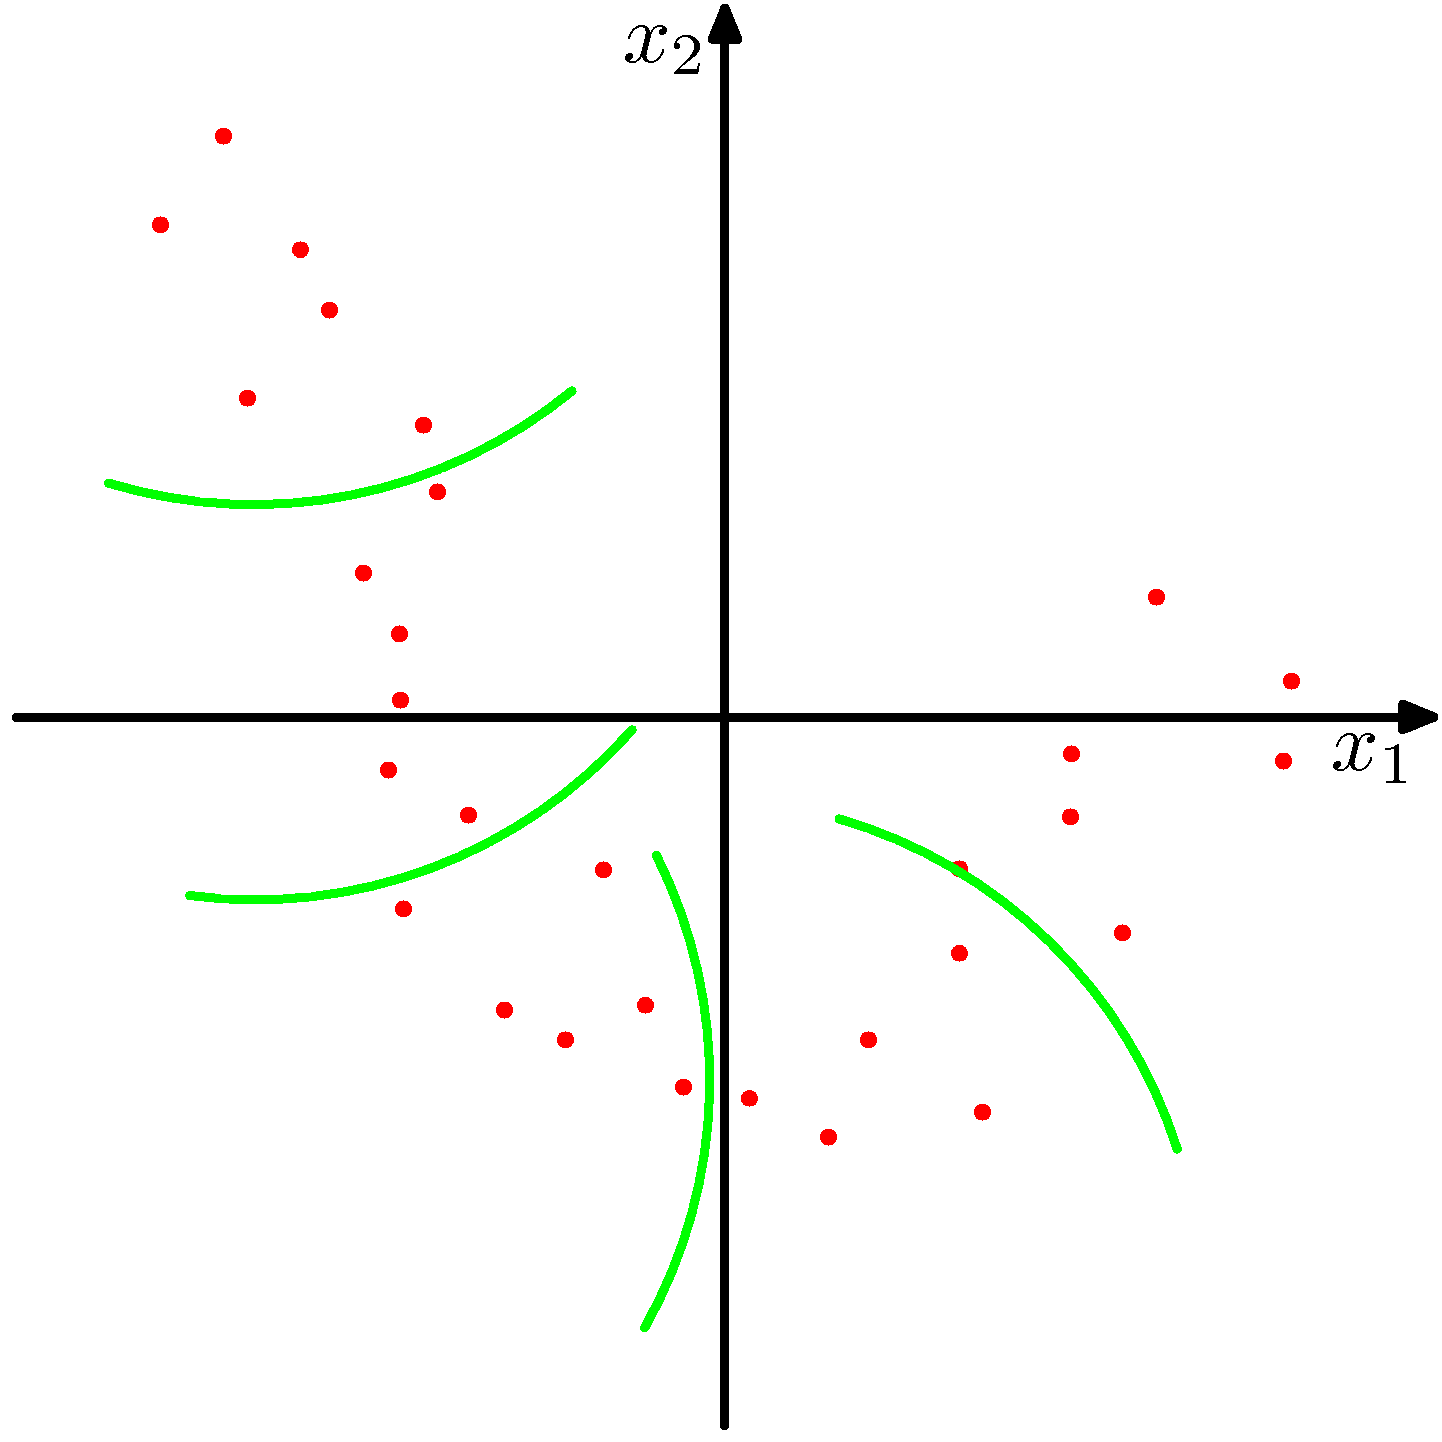
\includegraphics[width = 0.45\textwidth]{Chapter2/Figures/Figure12_16a.png}}\hfill
\subfloat[]{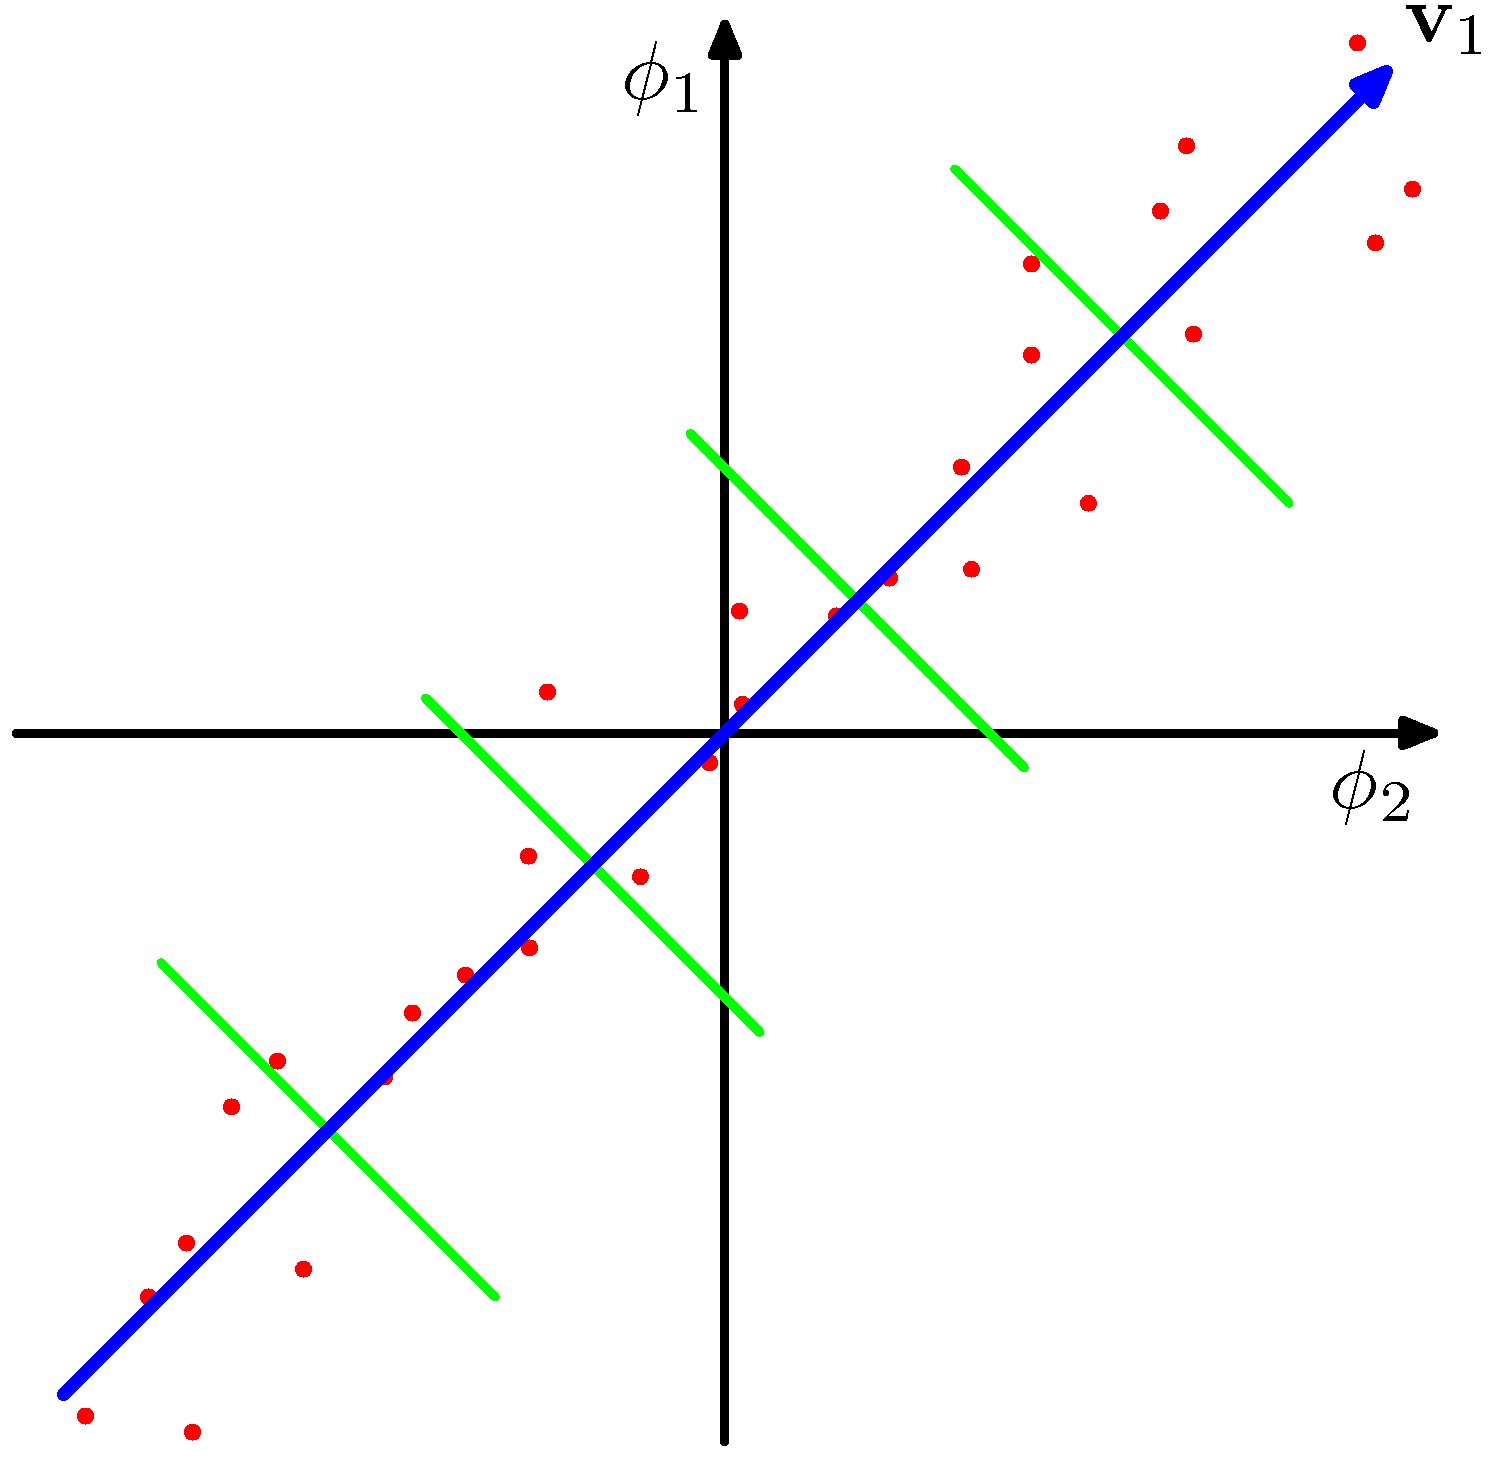
\includegraphics[width = 0.45\textwidth]{Chapter2/Figures/Figure12_16b.png}}
\caption[Kernel \ac{pca}]{Illustration of kernel \ac{pca}. (a) Nonlinear principal component in the original data space, (b) Nonlinear projection of the original data space into features space ($\phi(x)$).
In this space it is possible to apply linear \ac{pca}, $v_{1}$ is the first principal component in the feature space and the green lines are linear projections of the data to the principal component. This figure was taken from Bishop~et al.\,\cite{bishop2006pattern}.}
\label{fig:kpca}
\end{figure}   
Assuming that the projected data in the feature space is zero-mean, the covariance matrix in the feature space is given by: 
\begin{equation}
C_{M \times M} = \frac{1}{N}\sum\limits_{n=1}^{N} \phi(x_{n})\phi(x_{n})^{T}~.
\label{eq:Covkpca}
\end{equation}
Similar to the standard \ac{pca}, our goal is to find the eigenvectors of this matrix where the eigendecomposition is given by: 
\begin{equation}
\lambda_{i} v_{i} = C v_{i}.
\label{eq:edeckpca}
\end{equation}
Substituting Eq.~\ref{eq:Covkpca} in Eq.~\ref{eq:edeckpca}, the eigenvectors are given by: 
\begin{equation}
v_{i} = \sum_{n=1}^{N} a_{in}\phi(x_{n}).
\end{equation}
Using the previous formulation in the eigendecomposition, and based on the kernel substitution, the mapping in the feature space can be represented in terms of a kernel function $k(x_{n}, x_{m})$: 
\begin{subequations}
\begin{align}
\frac{1}{N}\sum\limits_{n=1}^{N} k(x_{l}, x_{n}) \sum\limits_{m=1}^{N} a_{im}k(x_{n}, x_{m}) & = \lambda_{i} \sum\limits_{n=1}^{N} a_{in}k(x_{l}, x_{n})~,\\
K a_{i} & = \lambda_{i}N a_{i},
\end{align}
\end{subequations} 
\noindent Here $a_{i}$ is an $N$-dimensional vector and $K$ is an $N \times N$ matrix solved by eigenvalue decomposition.
Based on the aforementioned equations, we can now formulate the principal component projections in terms of the kernel function as illustrated below: 
\begin{equation}
y_{i}(x) = \phi(x)^{T}v_{i} = \sum\limits_{n =1}^{N} a_{in}\phi(x)^{T}\phi(x_{n}) = \sum\limits_{n=1}^{N} a_{in}k(x,x_{n})~.
\end{equation} 

%\item \textbf{\acf{mvu}}
%\item \textbf{\acf{lle}}

\item \textbf{\acf{bow}} is a modeling or mapping of the extracted features to a new space based on a set of main clusters in the feature space. 
This method looks for similar or strong patterns among the extracted features and presents all the features based on the number of occurrence of these patterns. 
\Ac{bow} clusters a set of low-level features using a \textit{k}-means algorithm to create a ``codebook'' of ``visual words''.
Each visual word is defined by a centroid of the corresponding cluster. 
After creating the codebook, each sample is represented as a histogram of size \textit{k} obtained by calculating the occurrence frequency of the \textit{k} words among the features extracted from the sample.

K-means is an iterative algorithm that finds k centroids by alternating assignment and update steps.
The assignment steps are based on $L_{2}$ norm (Euclidean) distance.
Different initialization methods can be used in order to assign the initial \textit{k} clusters~\cite{celebi2013comparative}.
In this research, these clusters are selected based on the greedy \textit{k}-means++ method~\cite{arthur2007k}.
The choice of the visual words (number of \textit{k} clusters) depends on the application, and different choices can be made. 
A suitable number is usually found via an exhaustive search or primary tests.  


\item \textbf{\acf{scf}}, or sparse signal representation, has become very popular over the past few decades and has led to state-of-the-art results in various applications such as face recognition~\cite{wright2009robust}, image denoising, image inpainting~\cite{elad2006image}, and image classification~\cite{sidibe2015discrimination}. 
The main goal of sparse modeling is to efficiently represent the samples/images as a linear combination of a few typical patterns, called atoms, selected from the dictionary.
Sparse coding consists of three main steps: (i) dictionary learning, (ii) low-level feature projection, and (iii) feature pooling~\cite{rubinstein2008efficient}. 
Considering our dictionary $D \in R^{n \times K}$ with $K$ atoms, where each column of $D$ represents one atom, the sparse coding problem of a signal $y \in R^{n}$ is defined as finding the sparsest vector $x$ so that $y \approx Dx$. 
This is an optimization problem that can be formulated as:
\begin{equation}
\min_{x} \|y-Dx\|_{2} \qquad \text{s.t.}\ \|x\|_{0} \leq \lambda \,,
\end{equation}  
\noindent where $\lambda$ is the sparsity level and $l^{0}$-norm accounts for the minimum number of non-zero elements in the sparse vector $x$. 
This optimization problem is NP hard~\cite{Elad2010}, subsequently approximation solutions are proposed either by using greedy algorithms such as \ac{mp}~\cite{mallat1993matching} and \ac{omp}~\cite{davis1994adaptive}, or by replacing the $l^{0}$-norm with $l^{1}$-norm such as in the \ac{bp} algorithm~\cite{chen1998atomic}.
%\noindent where $\lambda$ is the sparsity level and $l^{0}$-norm accounts for the minimum number of non-zero elements in sparse vector $x$. 
%This optimization problem is NP hard~\cite{Elad2010}.
%Subsequently approximation solutions are proposed either by using greedy algorithms such as \ac{mp}~\cite{mallat1993matching} and \ac{omp}~\cite{davis1994adaptive} or by replacing the $l^{0}$-norm with $l^{1}$-norm such as \ac{bp}~\cite{chen1998atomic}.
The dictionary is learned using K-SVD, a generalized version of \textit{k}-means clustering that uses \ac{svd}~\cite{aharon2006img}. 
The dictionary is built such that:
\begin{equation}
  \min_{Dx} \|y - Dx\|_{2} \qquad  \text{s.t.} \ \forall i \ \|x_{i}\|_{1} \leq \lambda \,,
\end{equation}

\noindent where $y$ is a low-level descriptor, $x$ is the sparse coded descriptor (i.e., high-level descriptor) with a sparsity level $\lambda$, and $D$ is the dictionary with $K$ atoms.
The K-SVD algorithm solves the optimization problem iteratively by alternating between $x$ and $D$. 
With $D$, the sparse code matrix $x$ is computed by any of the pursuit algorithms, and with $x$, $D$ is updated one atom at a time using \ac{svd}. 

Once the dictionary is learned, each $y_{i} \in R^{n}$ signal can be projected using $D$ to form a set of sparse codes $x_{i} \in R^{K}$. 
In the case of image samples, the sparse representation can be generated for patches in the image.
In this case, the final mapping is based on a combination of sparse codes, for instance by taking the maximum code from all the patches: 
\begin{equation}
f_{i} = \max_{j}(\vert X_{l}(i,j)\vert) \qquad  \forall  i = 1, 2, .., K \,,
\end{equation} 
\noindent where $X_{l} \in R^{K \times P}$ is the sparse code matrix~\cite{sidibe2015discrimination}. 
\end{description}



%In this research we choose, feature representation approaches such as \ac{pca}, \ac{bow}, and \ac{scf}. 



%%% Local Variables: 
%%% mode: latex
%%% TeX-master: "../thesis"
%%% End: 

\section{Balancing Strategies} \label{sec:chp2-sec5}

While performing classification for real world applications, we usually face a problem in which the number of samples of one class is far less than the samples of another class.
This problem is frequently referred to as the ``class imbalance'' problem~\cite{prati2009data} and has been encountered in many diverse areas such as telecommunication management~\cite{ezawa1996learning}, bioinformatics~\cite{radivojac2004classification}, fraud detection~\cite{phua2004minority}, and medical diagnosis~\cite{celebi2007methodological}. 
Imbalanced data substantially compromises the learning process since most of the standard machine learning algorithms expect a balanced class distribution or an equal misclassification cost~\cite{he2009learning}.
Medical data are prone to such drawbacks due to the fact that the portion of diseased samples or patients is far lower than healthy cases.
Furthermore, the detection and classification of minority malignant cases is essential, so the \ac{se} of the algorithms developed needs to be maximized.
Consequently, the problem of imbalanced data is usually addressed by employing different techniques that do not impair the topology of the data.
This section discusses some of the most used balancing techniques.
%Despite the fact that classification of malignant melanoma has been extensively studied, up to our knowledge, only few works tackled the issue implied by imbalanced dataset~\cite{barata2013two,celebi2007methodological}.
%Barata~\emph{et al.} generate new synthetic samples by adding a Gaussian noise with fixed parameters to the samples belonging to the minority class~\cite{barata2013two}.
%Celebi~\emph{et al.} and Capdehourat~\emph{et al.} over-sampled their dataset using \ac{smote}~\cite{chawla2002smote} to improve the \ac{se} of their algorithm~\cite{celebi2007methodological, capdehourat2009pigmented}.

Considering a binary classification problem, the class with the smallest number of samples is defined as the \textit{minority} class and its counterpart is defined as the \textit{majority} class.
%The problem of data balancing corresponds to equalize the number of samples of both the minority and majority classes. This task can be achieved in either data or feature space.
%Balancing strategies in data space refers to elimination of some majority samples or generation of synthetic minority samples.
%Variation of the mean shapes, using \ac{pca}, in handwritten character recognition is an example of generation of synthetic data samples. 
%In feature space, three strategies can be employed to overcome the problem of imbalance dataset: (i) \acf{us}, (ii) \acf{os}, and (iii) a combination of both.
Data balancing corresponds to a sample number equalization in both the minority and majority classes. 
This task can be achieved either in the data or feature space.
Balancing strategies in the data space include elimination of some of the majority samples or the generation of synthetic minority samples. 
An example of synthetic sample generation in handwritten character recognition is the alteration of the mean character shapes using a \ac{pca}. 
In the feature space, three strategies can be employed to overcome the problem of imbalanced dataset: (i) \acf{us}, (ii) \acf{os}, and (iii) a combination of both.
The following sections give an overview of the techniques used to tackle this issue.

\subsection{\acl{us}}

The goal of \ac{us} is to reduce the number of samples from the majority class so that it is equal to the number of samples from the minority class.
The following methods are considered to perform the data balancing.

\begin{description}
  \item[\Ac{rus}] is performed by randomly removing a subset of samples from the majority class (without replacement) so that the number of samples is then equal in both classes.
  \item[\Ac{tl}] can be used to under-sample the majority class of the original dataset~\cite{tomek1976two}.
Let $(x_i, x_j)$ define a pair of \ac{nn} samples so their associated class labels are different $y_i \neq y_j$.
The pair $(x_i, x_j)$ is defined as a \ac{tl} if, by relaxing the class label differentiation constraint, there is no other $x_k$ sample defined as the \ac{nn} of either $x_i$ or $x_j$.
\Ac{us} is performed by removing the samples belonging to the majority class and forming a \ac{tl}.
It must be noted that this \ac{us} strategy does not enforce a strict balance between the majority and the minority classes.

  \item[\Ac{cus}] refers to the use of $k$-means to cluster the feature space so that $k$ is set to be equal to the number of samples composing the minority class.
Hence, the centroids of these clusters define the new samples from the majority class. 
 
  \item[\Ac{nm}] offers three different methods to under-sample the majority class~\cite{mani2003knn}.
%In \ac{nm1}, samples from the majority class are selected such that for each sample, the average distance to the $k$ \ac{nn} samples from the minority class is minimum.
%\ac{nm2} diverges from \ac{nm1} by considering the $k$ farthest neighbours samples from the minority class.
%In \ac{nm3}, a subset $M$ containing samples from the majority class is generated by finding the $m$ \ac{nn} from each sample of the minority class.
%Then, samples from the subset $M$ are selected such that for each sample, the average distance to the $k$ \ac{nn} samples from the minority class is maximum.
%In our experiment, $k$ and $m$ are fixed to 3.
 % \item[\Ac{enn}] is another \ac{us} approach, which removes any sample whose class label differs, at least, from the labels of two of its three \ac{nn}~\cite{wilson1972asymptotic}.
%This method removes samples from both majority and minority class both.      
In \ac{nm1}, for each selected sample in the majority class, the average distance to the $k$ \ac{nn} samples in the minority class is minimum.
\ac{nm2} diverges from \ac{nm1} by considering the $k$ farthest neighbour samples in the minority class.
\ac{nm3} generates a subset $M$ of the majority class samples by finding the $m$ \ac{nn}s of each minority class sample.
The elements in $M$ whose average distance to the $k$ \ac{nn} samples in the minority class is maximum are retained.
%In our experiment, $k$ and $m$ are fixed to 3. \textcolor{red}{Which experiment?}
  
  \item[\Ac{enn}] is another \ac{us} approach which removes any sample whose class label differs from the labels of at least two of its three \ac{nn}s~\cite{wilson1972asymptotic}.
This method removes samples from both the majority and minority classes.      
  \item[\Ac{ncr}] consists of applying two rules depending on the class of each sample~\cite{laurikkala2001improving}.
This is a modification of the (\ac{enn}) method that performs a better data cleaning.
Let us define $x_i$ as a dataset sample with its associated class label $y_i$, and $y_m$ as the class of the majority vote of the $k$ \ac{nn}s of $x_i$.
If $y_i$ corresponds to the majority class and $y_i \neq y_m$, $x_i$ is rejected from the final subset.
If $y_i$ corresponds to the minority class and $y_i \neq y_m$, then the $k$ \ac{nn}s are rejected from the final subset.
	
\end{description}

\subsection{\acl{os}}
Data balancing can also be performed by \ac{os}: new minority class samples are generated to equalize the number of samples in both classes.
Two different methods are considered.

\begin{description}
\item[\Ac{ros}] is performed by randomly replicating samples in the minority class so that the number of samples is equal in both the minority and majority classes.
\item[\Ac{smote}] is a method to generate synthetic samples in the feature space~\cite{chawla2002smote}.
Let us define $x_i$ as a sample belonging to the minority class, and $x_{nn}$ as a randomly selected sample from the $k$ \ac{nn}s of $x_i$.
Then \ac{smote} can generate a new $x_j = x_i + \sigma \left( x_{nn} - x_i \right)$ sample, where $\sigma$ is a random number in the interval $\left[0,1\right]$.

\end{description}

\subsection{Combination of \ac{os} and \ac{us}}

\ac{os} methods can be combined with \ac{us} to clean the newly generated over-sampled set of minority class samples.
In that regard, two different combinations are tested.

\begin{description}
  \item[\ac{smote} + \ac{tl}] are combined to clean the samples created using \ac{smote}~\cite{batista2003balancing, prati2009data}.
\Ac{smote} over-sampling may lead to overfitting, which can be avoided by removing the \ac{tl} from both the majority and minority classes.
%Thus, the \ac{tl} method is applied to the over-sampled training set to perform data cleaning and instead of removing only the majority samples with tomek-links, it removes samples from both classes~\cite{prati2009data}. 

  \item[\ac{smote} + \ac{enn}] ~\cite{batista2004study}.
The \acl{enn} removes all the misclassified samples with respect to its 3 \ac{nn}s, without any concern for their class, and generally eliminates more samples in comparison with \ac{tl}.
It is expected to have a more in-depth data cleaning when using \ac{enn}~\cite{prati2009data}.
\end{description}

Here, to deal with the imbalance problem, the fastest, simplest and least parametric heuristic \ac{os} and \ac{us} methods are discussed.
However, there are other approaches, such as ensemble and cost-sensitive learning, that are beyond our interest in this thesis.
A curious reader can refer to the following references~\cite{he2009learning,chawla2005data} for more information on this topic.


%%% Local Variables: 
%%% mode: latex
%%% TeX-master: "../thesis"

\section{Classification} \label{sec:chp2-sec6}
The classification problem was discussed previously in Sect.~\ref{sec:chp2-sec1}.
%We discussed and introduced the classification problem previously in Sect.~\ref{sec:chp2-sec1}. 
Numerous approaches have been introduced by the research community to solve the classification problem. 
%Here we will discuss some of these approaches under two categories of single learner and ensemble. 
Here we discuss some of these approaches divided into two categories: ``single learner'' and ``ensemble''.  

\subsection{Single Learner}
This group contains a large number of classifiers, or base learners, that have a unique approach to learn from the training set. 
In the following, we discuss some of these classifiers: \ac{svm}, K-\ac{nn}, \ac{lda} and \ac{nb}. 

\begin{description}

\item[\acf{nb}] is one of the simplest probabilistic classifiers, based on Bayes' theorem. 
This classifier has a ``naive'' or independence assumption that states that features are conditionally independent given the class variable~\cite{murphy2012machine}. 
Given a sample to be classified represented by $n$ features, $\mathbf{x} = (x_{1}, ..., x_{n})$, the conditional probability of this sample belonging to class $C_{k}$ based on Bayes' theorem is given by: 
\begin{equation}
p(C_{k}|\mathbf{x}) = \frac{p(C_{k})p(\mathbf{x}|C_{k})}{p(\mathbf{x})}.
\label{eq:BT}
\end{equation}
This equation simply states that the posterior is equal to the prior times the likelihood while normalized.
Considering that the numerator of Eq.~\ref{eq:BT} can be written as a joint probability $p(C_{k}, x_{1}, ..., x_{n})$ and taking into account the conditional independence assumption, the \ac{nb} model is represented by: 
\begin{equation}
p(C_{k}|x_{1}, ..., x_{n}) = \frac{1}{Z}p(C_{k})\prod_{i =1}^{n} p(x_{i}|C_{k}),
\label{eq:nbM}
\end{equation} 
\noindent where $Z = p(x)$ is the normalization or scaling factor depending on $x_{1}, ...,x_{n}$.
For classification purposes, the \ac{nb} is combined with decision rules, such as \acf{map} or \acf{ml}: 
\begin{equation}
\hat{y} = \argmax_{k\in\{1,...,k\}} p(C_{k})\prod_{i=1}^{n} p(x_{i}|C_{k})~.
\end{equation}  

\item[K-Nearest Neighbor (k-\ac{nn})] is another simple and non-parametric classification method. 
This classifier assigns each sample's label based on the majority vote of its $K$ nearest neighbors. 
If $K$ is equal to 1, the output is assigned to the label of the nearest neighbor.
   
\item[\acf{lda}] or the Fisher linear discriminant analysis, was introduced in Sect.~\ref{sec:chp2-sec4} as a dimension reduction approach that takes the class label into account. 
Since this method contains the class information, it can be used for classification as well. 
However, it has a drawback, that regardless of the number of feature dimensions, it always maps the data to $L\leq C-1$. 
%Which indicates that for two class classification, it maps the data to one vector where the class margin is maximized~\cite{murphy2012machine}. 
This indicates that for a two class classification, in an attempt to maximize the margin between the two class, it maps the data to one vector~\cite{murphy2012machine}.

\item[\acf{svm}] is created based on the combination of the kernel trick and modified loss function~\cite{murphy2012machine}.
\ac{svm}~\cite{vapnik1963generalized} is a well known machine learning approach that aims to separate two classes by finding the best hyperplane maximizing the margin between the two classes: 
\begin{equation}
\min\limits_{\mathbf{w},\omega_{0}, \mathbf{\xi}} \frac{1}{2} \Vert \mathbf{w} \Vert^{2} + C \sum\limits_{i = 1}^{N} \xi_{i} \qquad \text{s.t. } \quad \xi_{i} \geq 0, \quad y_{i}(x_{i}^{T}\mathbf{w} + \omega_{0}) \geq 1 - \xi_{i}, i = 1:N .
\label{eq:svmop}
\end{equation}

Maximizing the margin is equivalent to minimizing the norm of the normal vector of the hyperplane: 
% Soft margine  no points should lie in the margin and can be solved as an optimization problem. 
\begin{equation}
\min\limits_{\mathbf{w}, \omega_{0}} \frac{1}{2} \Vert \mathbf{w}\Vert^{2} \qquad \text{s.t. } \quad  y_{i}(\mathbf{w}^{T}\mathbf{x_{i}} + \omega_{0}) \geq 1, i = 1: N.
\label{eq:svmsm}
\end{equation}
\noindent This constraint intends to force all the points to be on the correct side of the decision boundary (hyperplane) with a minimum distance of 1. 
This assumption is only valid if the data is linearly separable. 
Thus, for general cases, a slack variable $\xi_{i} \geq 0 $ is introduced. 
If the points are on/or inside the correct margin boundary, then $\xi_{i} = 0 $; if the points are inside the margin and still on the correct side of the decision boundary, then $0 < \xi_{i} \leq 1 $; otherwise, if the points lay on the wrong side of the decision boundary, $\xi_{i} > 1 $. 
This assumption introduces \textit{soft margin constraints}.
Considering the rule of $\xi_{i}$, the $\sum_{i} \xi_{i}$ term in Eq.~\ref{eq:svmop} describes the upper bound on the number of misclassified points and $C$ is the regularization parameter that controls the tolerance of the classifiers on the number of errors~\cite{murphy2012machine}. 
\end{description}  
   
\subsection{Ensemble}
Ensemble learners are defined by a combination of several base learners $f_{m}(.)$:
\begin{equation}
f(y|y, \pi) = \sum\limits_{m\in M} \omega_{m}f_{m}(y|x),
\label{eq:ensmeble}	
\end{equation} 
\noindent where $\omega_{m}$ is the tunable parameter~\cite{murphy2012machine}. 
Some ensembles are created based on the combination of base learners of the same type, such as \acf{rf} and \acf{adb}, whereas others combine different base learners in a specific way, e.g. stacking and \acf{ecoc}. 
Some well-known ensembles are described in the following. 

\begin{description}
\item[\acf{adb}] (short for Adaptive Boosting) is an ensemble learning algorithm that provides a high performance classifier via a linear combination of weak learners~\cite{freund1996experiments}.
Considering a training set $(x_{i}, y_{i})$, where $x$ is an $M$ dimensional feature vector and $y_{i}$ is its associated class label, \ac{adb} iteratively adds weighted weak learners ($\alpha_{t}h_{t}$) to assemble the final strong classifier.
Here, $\alpha_{t}$ is the weight and $h_{t}$ is the weak learner:
\begin{equation}
H(x) = sign (\sum\limits_{t =1}^{T} \alpha_{t}h_{t}(x))~.
\label{eq:adb}
\end{equation}
A weak learner is usually selected as a classifier that performs slightly better than randoms ($> 50\%$).
Weak learners are selected with their associated weight so that the sum of the training error $E_{t}$ of the resulting $t$ stage classifier is minimized. 
\begin{subequations}
\begin{align}
E_{t} &= \sum\limits_{i = 1}^{N} e^{-y_{i}H_{t}(x_{i})}~,\\
H_{t}(x) &= \alpha_{1}h_{1}(x) + ...+\alpha_{t}h_{t}(x)~.
\end{align}
\label{eq:adberror}
\end{subequations}
This ensemble is constructed with the aim of classifying harder patterns by re-weighting the distribution after each iteration~\cite{rokach2010ensemble}. 
Starting with equally distributed weights for our distribution $D_{1}(i) = 1/N, \quad i = 1: N$.
The distribution is updated after each iteration in a manner that the weights of correctly classified samples decrease and the weights of misclassified samples increase. 
\begin{equation}
D_{t+1}(i) = \frac{D_{t}(i).e^{-\alpha_{t}y_{t}h_{t}(x_{i})}}{Z_{t}}~.
\end{equation}
Re-weighting the distribution automatically forces the next weak learner to focus on the difficult samples.  
As mentioned previously, each weak learner is assigned a weight as well and the best weak learners have higher weights in comparison to the weakest learners.

A variety of learners can be adapted in the algorithm as weak learners such as neural networks or decision trees. 
One common weak learner is decision stump, which is a one-level decision tree, equivalent to the threshold that best splits the data.  
Each stump learner is characterized by three parameters: (i) the $m^{th}$ dimension of the features set where the classifier is applied, (ii) the decision level, i.e., the threshold splitting the data in the $m^{th}$ given dimension and (iii) the decision sign ($-$1 or +1) determining the inequality direction for the thresholding.
For a given batch of data with a set of features of size $M$, at each iteration of \ac{adb}, the decision stump that minimizes the error $t$ in an $m^{th}$ dimension of the training distribution is selected.
The information provided by the final set of decision stumps selected by \ac{adb} can also be used for determining the significant features of the data-stream and, more importantly the best split in the data.

\item[\acf{rf}] is an ensemble of decision trees~\cite{breiman2001random} that generalizes the classification process by applying two types of randomization: at the tree level, each tree is fed by a bootstrap made of $S'$ samples build from the original data of size $S$ so that  $S=S'$, and at the node level, a subset of feature dimensions $m$ is randomly selected from the original dimension $M$ so that $m=\sqrt{M}$. 
The trees in \ac{rf} are grown to their maximum length without any pruning.
Figure~\ref{fig:rftrain} shows the training stage of an \ac{rf} ensemble.
In this figure rows and columns represent the samples and the feature dimensions, respectively.
As it mentioned each tree is trained on the bootstrap of the original samples and in each node of a tree, subset of feature dimensions are used for prediction.  
In the testing stage, each tree in the ensemble casts a unit vote, and the final prediction is based on the combination of all the votes.
This process is shown in Fig~\ref{fig:rftest}.
\begin{figure}
\centering
\subfloat[]{
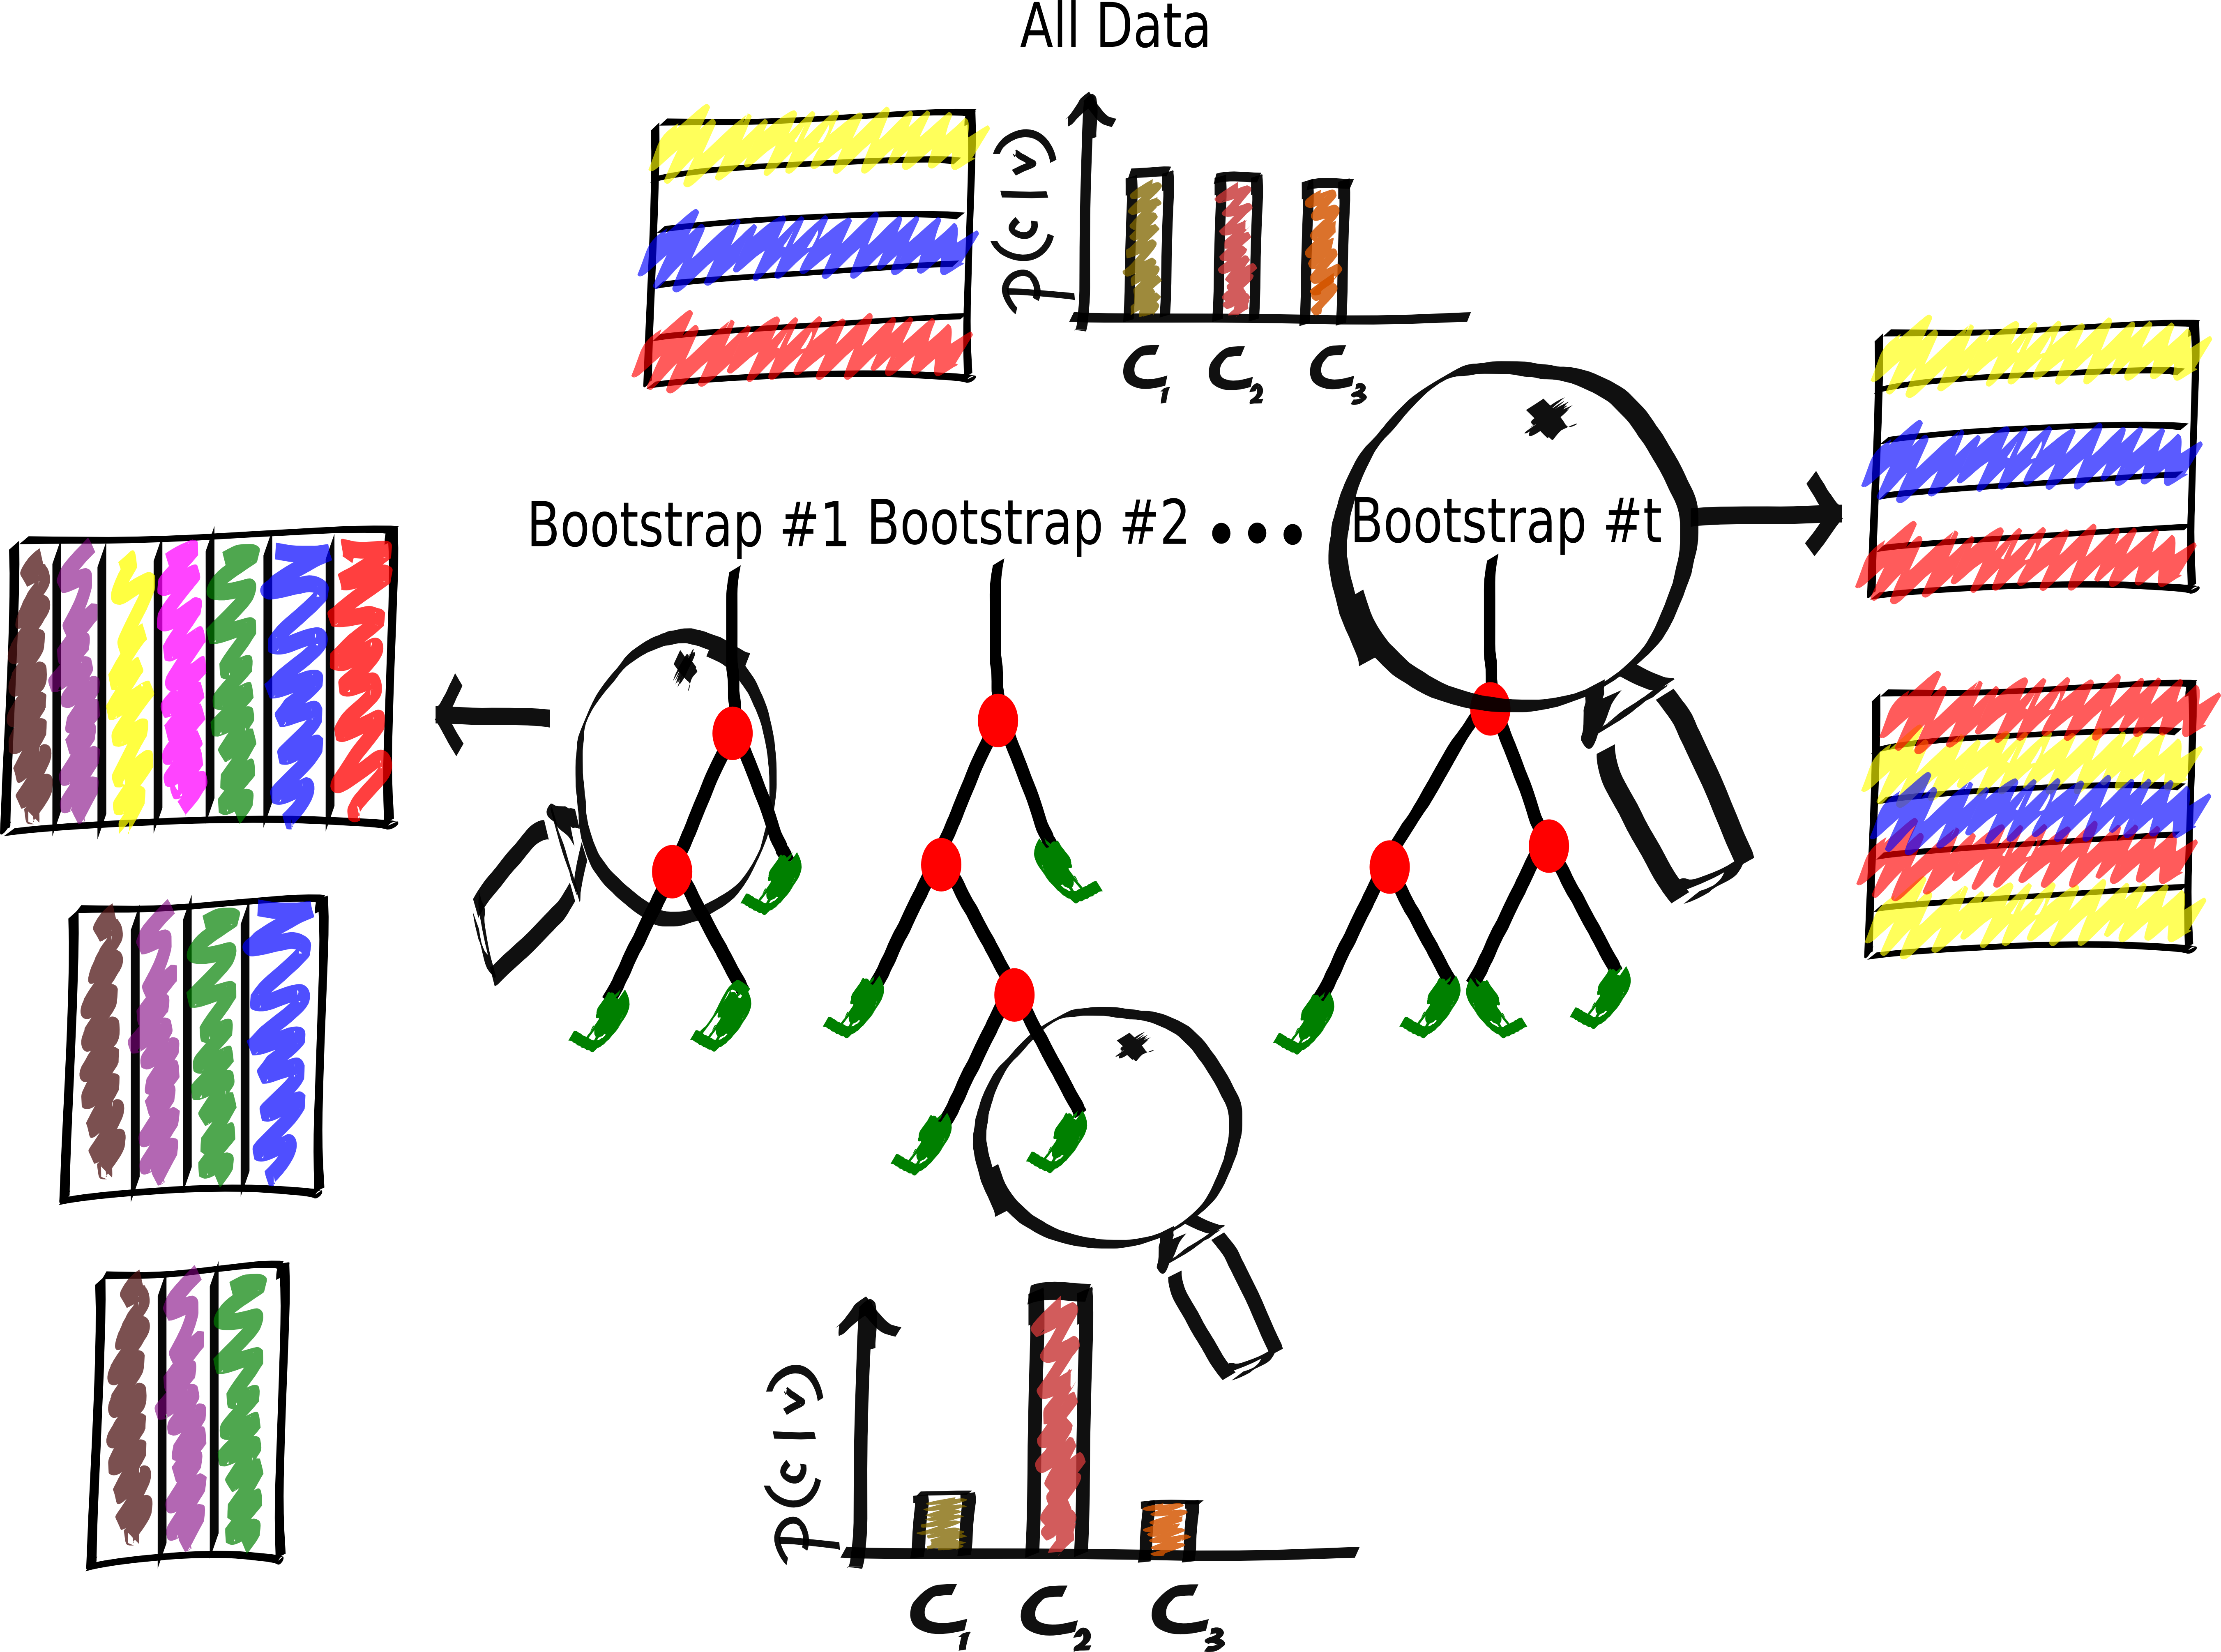
\includegraphics[width = 0.8\textwidth, height = 0.4\textheight]{Chapter2/Figures/RF_train.png}
\label{fig:rftrain}}\\
\subfloat[]{
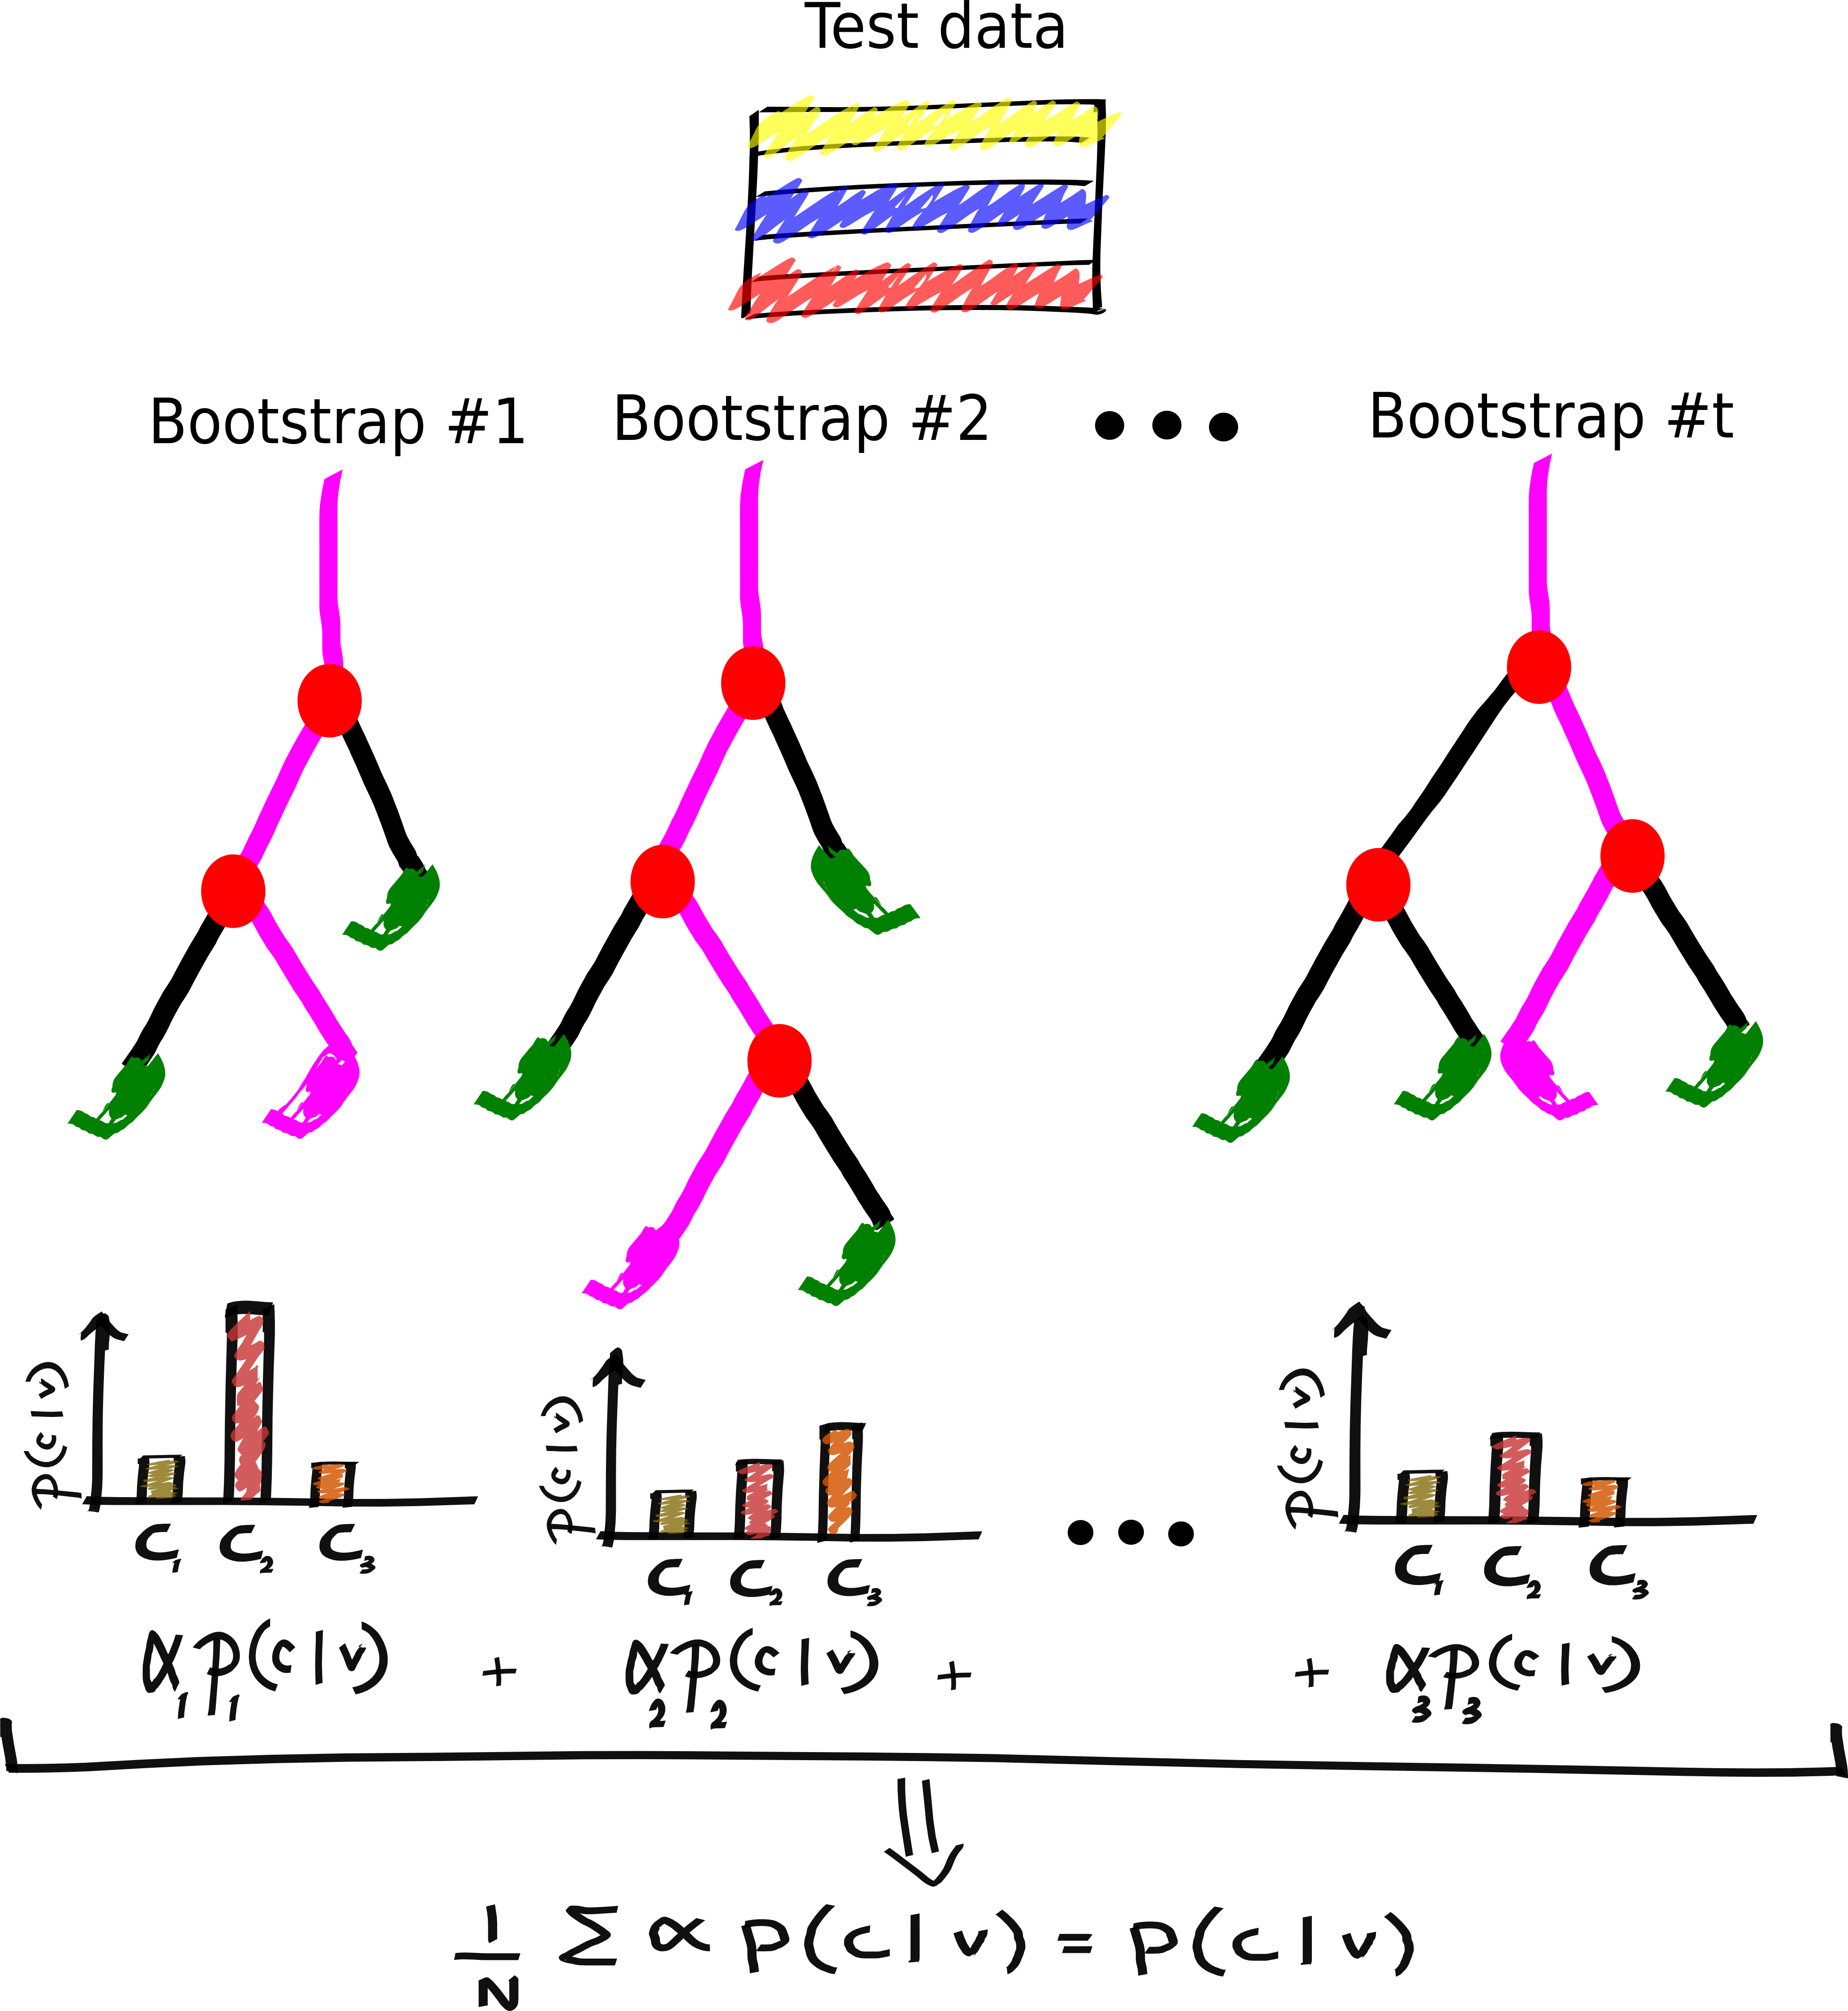
\includegraphics[width = 0.5\textwidth, height = 0.4\textheight]{Chapter2/Figures/RF_test.png}
\label{fig:rftest}}
\caption[\acl{rf} classifier]{\Ac{rf} ensemble: (a) training stage of \ac{rf} ensemble. This ensemble randomizes the training by first creating different bootstraps for training each tree in the forests. Second, at each node of the tree, it randomly considers a smaller set of feature dimensions. Each node of a tree predicts one class. (b) testing stage of \ac{rf} ensemble. A test sample is passed through all the trees and its prediction is assigned by majority voting of predicted labels of the trees.}
\label{fig:rf}
\end{figure}

 
\item[\acf{gb}] is a generalization form of \ac{adb} able to use real-value weak learners and minimize different loss functions~\cite{zheng2007general}.
\ac{gb} builds the ensemble in a greedy manner. 
It iteratively selects the best pair of real-valued weak learners and adjusts their weights so they minimize a given differentiable loss function.
\begin{subequations}
\begin{align}
\mathcal{L} & = \sum\limits_{i = 1}^{N} L(y_{i}, \varphi(x_{i})),\\
\varphi(x) & = \sum\limits_{j = 1}^{M} \alpha_{j} h_{j}(x),
\end{align}
\end{subequations}
\noindent here $h_{j}(.)$ is the weak learner and $\alpha_{j}$ is the real value weight and the aim is to minimize $\mathcal{L}$. 
A common choice for the weak learner is a decision stump or regression tree while the loss function is generally an exponential or a logarithmic loss~\cite{becker2013supervised}. 
\begin{subequations}
\begin{align}
\text{Exponential loss } \qquad L &= e^{-y_{i}\varphi(x_{i})}, \label{eq:exploss} \\ 
\text{Log loss } \qquad L &= \log(1+e^{-2y_{i}\varphi(x_{i})}).
\end{align}

\end{subequations}
This minimization can be carried out via a gradient descent or a quadratic approximation.

\item[Stacking]~\cite{wolpert1992stacked} is another way to create an ensemble from multiple base learners.
The idea is to have a meta learner which considers the predictions of the previous base learners as input for the training stage and combines them into a final decision.
Using this technique, the training data is partitioned into two sets, which we call training and validation sets. 
Each base learner is trained on the training set and its prediction on the validation set is fed to the meta learner.
Similarly, the test sample is first classified by the base learners and their prediction is passed through the meta learner in order to arrive at the final decision.
Stacking seems to avoid overfitting and improves performance when it is used with cross-validation~\cite{dvzeroski2004combining}.
This technique was used for problems such as segmentation and labeling~\cite{murphy2012machine}.
Figure~\ref{fig:stacking} shows the principal of the staking approach. 
\begin{figure}[t]
\centering
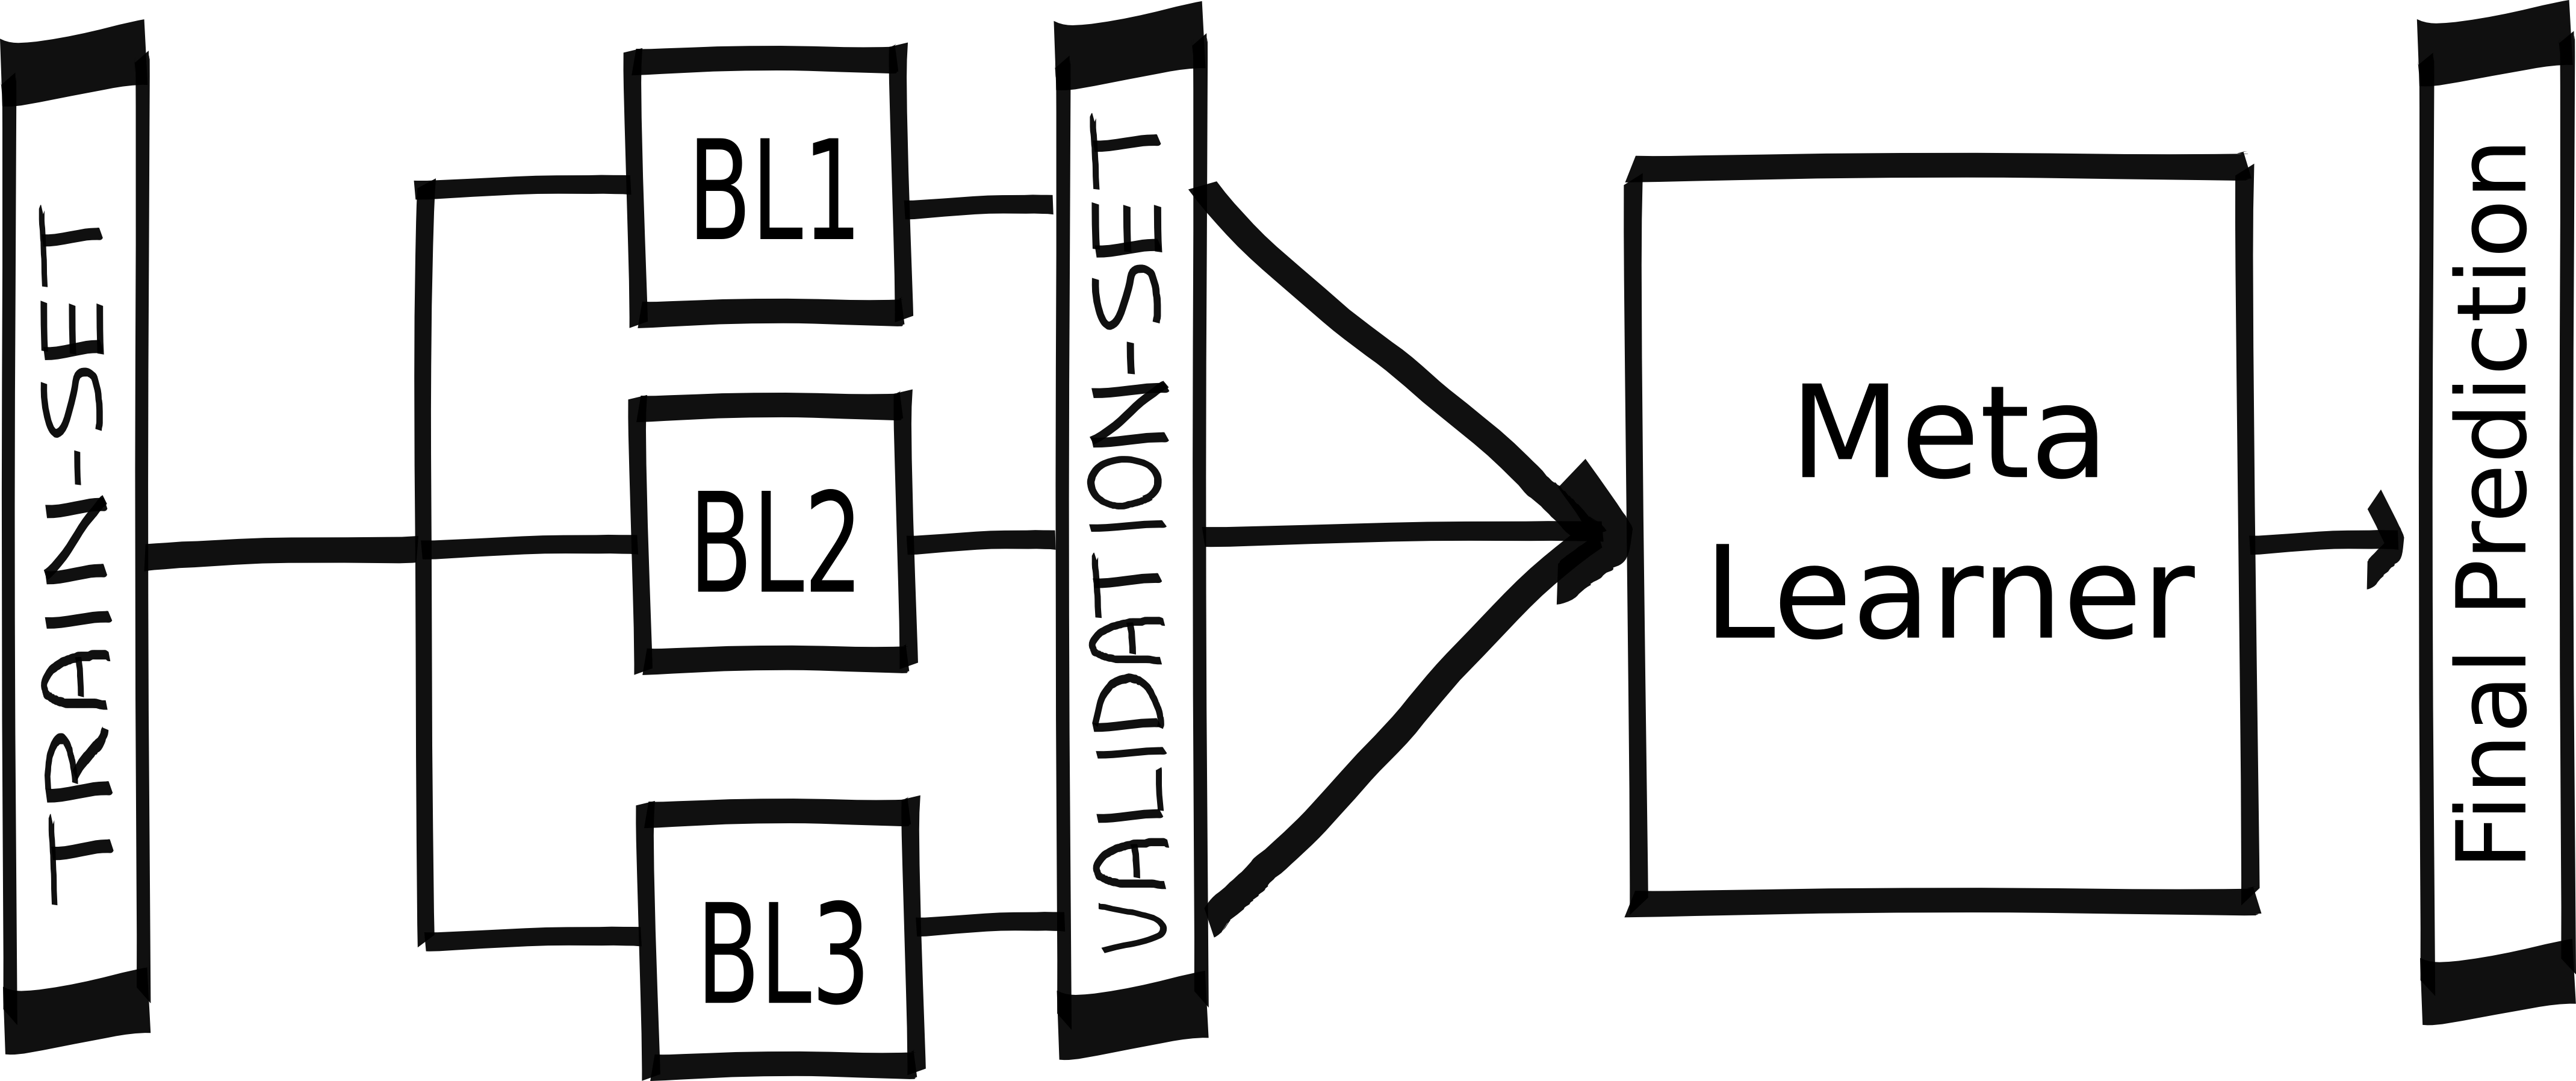
\includegraphics[width = 0.5\textwidth]{Chapter2/Figures/Stacking.png}
\caption[Stacking ensemble]{Staking ensemble approach for three base learners (BL1, BL2, and BL3). Different base learners can be combined using this method.}
\label{fig:stacking}
\end{figure}

\item[\acf{ecoc}] is an interesting way of ensemble learning, especially suitable for multiclass classification~\cite{dietterich1995solving}.
This technique allows the application of binary classifiers for multiclass classification by randomly assigning different classes to a ``super-class'' (0 or 1). 
Let us consider a 5 class classification $C \in \{A,B,D,E,F\}$, each time a set of classes is randomly assigned to one of the super-classes.
For instance, lets consider a binary classifier, where $A$ and $F$ are categorized in super-class 1 and $B$,$D$, and $E$ belong to super-class 0. 
Repeating the binary classification several times, each class will be represented by a binary code. 
This binary code states that in each binary classification, our considered class was categorized in one or the other super-class. 
Going back to our example and assuming a 5 binary classification, having a binary code $11010$ for class $F$ shows that for binary classification problems of 1,2, and 4, $F$ was assigned to super-class 1 and the rest to 0. 
Subsequently, an ensemble is created as a combination of binary classifiers.
Similarly, a test sample is classified with all the binary classifiers and receives a predicted binary code.
The predicted class is assigned based on the closest class vector to the predicted vector. 
Hamming distance is used to find a closest class vector. 
Although the classes can be assigned in a pre-designed manner to maximize their distance to each other, James~et. al~\cite{james1998error} showed that the random code works just as well as the optimal code~\cite{murphy2012machine}. 
%{\color{blue} Eventually if the created code vector is long enough, the effect of randomness is not feasible.}

\item[Weighed combination] is a very simple way of ensemble learning, and, as its name suggests, it creates a weighted combination of base learners.
Each base learner will have a strength proportional to its assigned weight.
The assigned weight can be fixed or dynamically determined.
There are different approaches to determine the base learners' weights: majority voting (plurality vote), Bayesian combination, entropy weighting and performance weighting among others~\cite{rokach2010ensemble}.
Each base learner's weight is proportional to the aforementioned measures on the validation set.
Figure~\ref{fig:LC_general} shows an ensemble based on performance weighting of three base learners (BL). 
\begin{figure}
\centering
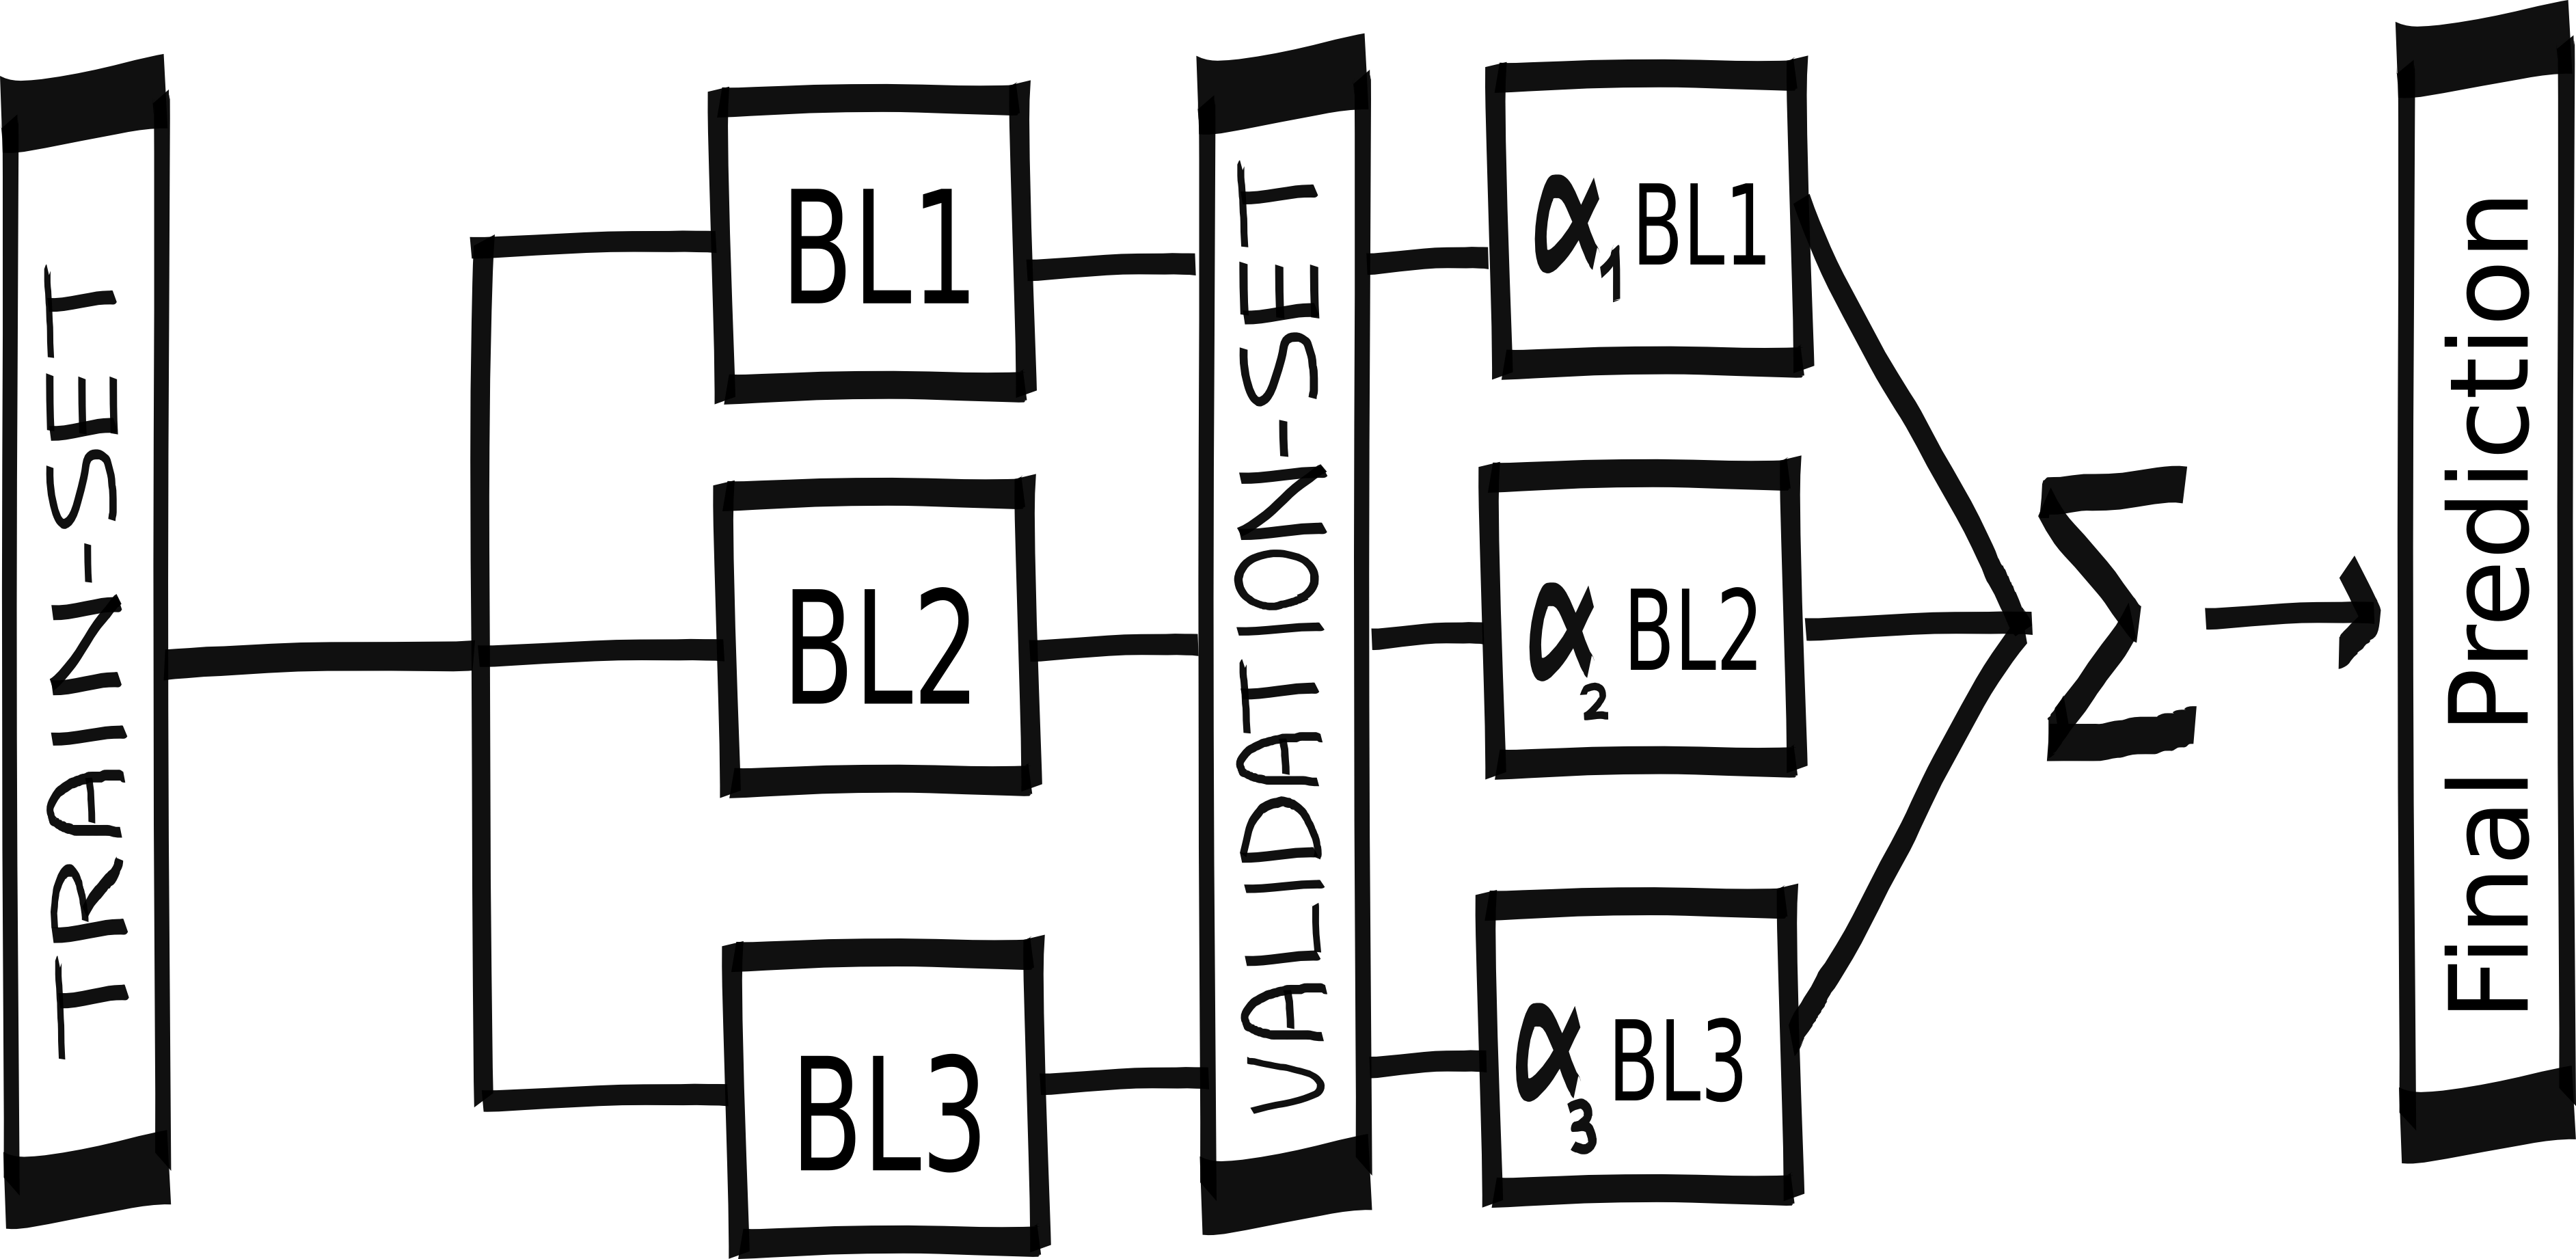
\includegraphics[width = 0.5\textwidth]{Chapter2/Figures/LC_gen.png}
\caption[Weighted Combination ensemble]{An ensemble of three base learners (BL1, BL2, and BL3, respectively) weighted by their performance on the validation.}
\label{fig:LC_general}
\end{figure} 
\end{description}



%%% Local Variables: 
%%% mode: latex
%%% TeX-master: "../thesis"
%%% End: 

\section{Validation and Evaluation} \label{sec:chp2-sec7}
This section first discusses different methods of validation and then presents different measurements of validation. 
\subsection{Validation}
Validation, or cross-validation, is an important part of the classification framework that ensures its generalization.
Validation also avoids having a bias classifier or overfitting. 
\acf{kcv} and \acf{loocv} are two different techniques for performing validation. 
In this section, we first discuss different methods for validation of a data classification framework and then present various measurements of its evaluation. 

\acl{kcv} randomly divides the dataset into $k$ partitions of equal size.
Among the $k$ partitions, one is used as the test set, and the classifier is trained on the remaining $k-1$ subsets. 
Using \ac{kcv}, the classification is performed $k$ times to ensure that each of the subsets is used as the test set once.

Leave-one-out-cross-validation can be seen as a form of \ac{kcv} when $k = n$, n is the total number of samples.
In this validation, the classification is repeated $n$ rounds. 
At each round, one sample is left out for testing and the classifier is trained on the remaining samples.
This method is suitable when dealing with a small or unbalanced dataset.    

\subsection{Evaluation}
Evaluation is another important part of the framework that measures the quality and performance of the framework.
While solving classification problems, a simple way to quantify the performance of the classifier is to look at the confusion matrix.
The confusion matrix is an error table that shows the performance of the algorithm.
Each row of the matrix represents instances in the predicted class and each column shows instances in their actual class (or vice-versa). 
Figure~\ref{fig:CM} shows the table and graphical representation of a confusion matrix.

\colorlet{circle edge}{blue!50}
\colorlet{circle area}{blue!20}


% Definition of circles
% \def\myRadius{1.5cm}
% \def\vennSpace{(0,0) rectangle (6cm,4cm)}
% \def\predictedCircle{(2cm,2cm) circle (\myRadius)}
% \def\actualCircle{(4cm,2cm) circle (\myRadius)}
% \def\myLabelRadius{1.3cm}

\def\myRadius{.75cm}
\def\vennSpace{(0,0) rectangle (3cm,2cm)}
\def\predictedCircle{(1cm,1cm) circle (\myRadius)}
\def\actualCircle{(2cm,1cm) circle (\myRadius)}
\def\myLabelRadius{.60cm}

\tikzset{fillbase/.style={fill=circle area, draw=circle edge, thick},
         filled/.style={pattern=crosshatch dots, draw=circle edge, thick},
         outline/.style={draw=circle edge, thick}}

\def\drawPredicted{
    \draw[outline] \predictedCircle node (x){}; % {$\bullet$};
    \node [above left=\myLabelRadius of x, anchor=center, outer sep=0](p){$P$};
    \node  at (p.300) {$+$};
    \node  at (p.120) {$-$};
}

\def\drawActual{
    \draw[outline] \actualCircle node (x){}; % {$\bullet$};
    \node [above right=\myLabelRadius of x, anchor=center, outer sep=0](a){$A$};
    \node  at (a.60) {$-$};
    \node  at (a.240) {$+$};
}

% Define the different metrics: tp, tn, fp, fn
\def\tp{
      \draw[outline] \vennSpace;
      \begin{scope}
        \clip \predictedCircle;
        \fill[filled] \actualCircle;
      \end{scope}
      \drawPredicted
      \drawActual
      % \draw[outline] (current bounding box.south west)
      %   rectangle (current bounding box.north east);
}

\def\tn{
      \draw[outline] \vennSpace;
  \begin{scope}[even odd rule]
    \fill[filled] \vennSpace
      \actualCircle
      \predictedCircle;
    \clip \actualCircle;
    \fill[white] \predictedCircle;
  \end{scope}
  \drawPredicted
  \drawActual
}

\def\fp{
      \draw[outline] \vennSpace;
      \begin{scope}
        \clip \predictedCircle;
        \fill[filled, even odd rule]
              \predictedCircle \actualCircle;
      \end{scope}
      \draw[outline] \vennSpace;
      \drawPredicted
      \drawActual
}

\def\fn{
      \draw[outline] \vennSpace;
      \begin{scope}
        \clip \actualCircle;
        \fill[filled, even odd rule]
              \actualCircle \predictedCircle;
      \end{scope}
      \draw[outline] \vennSpace;
      \drawPredicted
      \drawActual
}

\def\se{
  \fill[fillbase] \actualCircle;
      \begin{scope}
        \clip \predictedCircle;
        \fill[filled] \actualCircle;
      \end{scope}
      \draw[outline] \vennSpace;
      \drawPredicted
      \drawActual
}


\def\sp{
  \fill[fillbase, even odd rule]
    \vennSpace \actualCircle;
  \begin{scope}[even odd rule]
    \fill[filled] \vennSpace
      \actualCircle
      \predictedCircle;
    \clip \actualCircle;
    \fill[white] \predictedCircle;
  \end{scope}
  \draw[outline] \vennSpace;
  \drawPredicted
  \drawActual
  }


\begin{figure}[t]
  \def\myRadius{.65cm}
  \def\vennSpace{(0,0) rectangle (2.6cm,1.6cm)}
  \def\predictedCircle{(.8cm,.8cm) circle (\myRadius)}
  \def\actualCircle{(1.8cm,.8cm) circle (\myRadius)}
  \def\myLabelRadius{.450cm}
\centering{
\subfloat[]{
%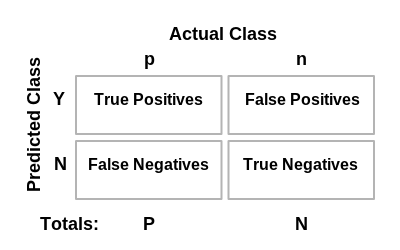
\includegraphics[scale= 0.3]{Chapter2/Figures/confusion-matrix_1.png}}\hfill
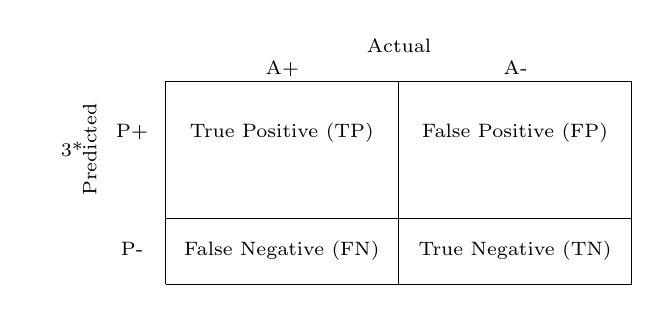
\begin{tikzpicture}[scale=0.4]
      \node at (0,0){
      \scriptsize{
        \begin{tabular}{
            >{\centering}m{1em} >{\centering}m{1em} >{\centering}m{1in} >{\centering\arraybackslash}m{1in}}
          % c>{\centering}m{2em}ccc}
          & & \multicolumn{2}{c}{ Actual}\\
          & & A+ & A- \\
          \cline{3-4}
          & \multicolumn{1}{c|}{} & \multicolumn{1}{c|}{} & \multicolumn{1}{c|}{}\\
          \multirow{3}{*}{\rotatebox[origin=c]{90}{Predicted}}& \multicolumn{1}{c|}{P+} &  \multicolumn{1}{c|}{True Positive (TP)} & \multicolumn{1}{c|}{False Positive (FP)} \\
          &\multicolumn{1}{c|}{}  & \multicolumn{1}{c|}{}& \multicolumn{1}{c|}{} \\
          \cline{3-4}
          & \multicolumn{1}{c|}{} &\multicolumn{1}{c|}{} & \multicolumn{1}{c|}{}\\
          
          & \multicolumn{1}{c|}{P-} &\multicolumn{1}{c|}{False Negative (FN)}  &\multicolumn{1}{c|}{True Negative (TN)}\\
          & \multicolumn{1}{c|}{} &\multicolumn{1}{c|}{} & \multicolumn{1}{c|}{}\\
          \cline{3-4}
          \end{tabular}
      }};
    \end{tikzpicture}
    }\\

  \subfloat[]{
    \label{fig:evaluation-confusion_matrix}
    \begin{tikzpicture}[scale=0.4]
      \node at (0,0){
        \begin{tabular}{
            >{\centering}m{1em} >{\centering}m{1em} >{\centering}m{1in} >{\centering\arraybackslash}m{1in}}
          % c>{\centering}m{2em}ccc}
          & & \multicolumn{2}{c}{ Actual Class }\\
          & & A+ & A- \\
          % \parbox[t]{2mm}{\multirow{2}{*}{\rotatebox[origin=c]{90}{\usebox \centering Predicted Class}}}& P+ &  \tikz{\tp} & \tikz{\fp} \\
          \multirow{3}{*}{\rotatebox[origin=c]{90}{Predicted Class}}& P+ &  \tikz{\tp} & \tikz{\fp} \\
          & P- & \tikz{\fn} & \tikz{\tn}
        \end{tabular}
      };
    \end{tikzpicture}
  }
  }
  \caption[Confusion matrix]{Tabular (a) and graphical (b) representations of a confusion matrix with true and false positive samples (\acs{tp}, \acs{fp}) in the first row and false and true negative samples (\acs{fn}, \acs{tn}) in the second row (from left to right).}
  \label{fig:CM}
\end{figure}
True positive (\ac{tp}) and \acf{tn} instances are simply the samples that are correctly predicted to belong to the positive or negative class, respectively.
False positive (\ac{fp}) samples are predicted as the positive class while in reality they belong to the negative class; and \acf{fn} instances are predicted as the negative class while belonging to the positive class.
Various statistic measures are derived form the confusion matrix, among which the most popular ones are \acf{acc}, \acf{se}, \acf{sp}, and precision.

Accuracy (see Eq.~\ref{eq:acc}) measures the overall performance of the algorithm by considering the number of instances classified correctly without considering their classes.
Although this measure is important, it can be misleading in real-world classification problems because an overfitted or biased classifier can have high accuracy while not performing as desired.
\begin{equation}
\ac{acc} = \frac{TP+TN}{TP+TN+FP+FN}~.
\label{eq:acc}
\end{equation} 
The sensitivity, recall or true positive rate is another statistic that measures an performance of the algorithm with respect to the positive class only.
\begin{equation}
\ac{se}	 = \frac{TP}{TP+FN}~.
\label{eq:se}
\end{equation}
Opposite to \ac{se}, \acl{sp} or true negative rate measures the algorithm's performance with respect to the negative class:
\begin{equation}
\acs{sp} = \frac{TN}{TN+FP}.
\label{eq:sp}
\end{equation}
Figure~\ref{fig:sesp} shows a graphical illustration of \ac{se} and \ac{sp} in the confusion matrix.
\begin{figure}
 \def\myRadius{.65cm}
 \def\vennSpace{(0,0) rectangle (2.6cm,1.6cm)}
 \def\predictedCircle{(.8cm,.8cm) circle (\myRadius)}
 \def\actualCircle{(1.8cm,.8cm) circle (\myRadius)}
 \def\myLabelRadius{.450cm}
  
\centering
\begin{tikzpicture}[scale=0.5]
      \def\seEquation{$SE = \frac{TP}{TP+FN}$}
      \def\spEquation{$SP = \frac{TN}{TN+FP}$}
      \node[label={[]below:\seEquation}](se){\tikz{\se}};
      \node[right=5pt of se, label={[]below:\spEquation}]{\tikz{\sp}};
      %\node[label={[]right:\seEquation}](se){\tikz{\se}};
      %\node[below=5pt of se, label={[]right:\spEquation}]{\tikz{\sp}};
\end{tikzpicture}
    
\caption[Sensitivity and Specificity]{Sensitivity and \acl{sp} evaluation, corresponding to the ratio of the doted area over the blue area.}
\label{fig:sesp}
\end{figure}

Precision or positive predictive value (PPV), as its name suggests, is a measure of the algorithms precision.
Considering an algorithm that is more biased towards the positive class, this algorithm has high \ac{se}, however, it is less precise, since it considers most of the instances as more or less positive.
\begin{equation}
precision = \frac{TP}{TP+FP}~.
\label{eq:ppv}
\end{equation} 

All the aforementioned measures can be used to quantify the performance of an algorithm.
They can also be combined to generate a graphical plot such as \acf{roc} or precision-recall curve.
The \ac{roc}~\cite{zweig1993receiver} is a graphical curve of \ac{se} against a \acf{fpr} or (1 - \ac{sp}).
The curve is constructed by varying the discriminant threshold of the classifier.
Adjusting the threshold will lead to classifying more \ac{tp} samples, usually at the cost of increasing \ac{fp}s.
Due to this property, the \ac{roc} is a valuable tool, specially in the medical field when having high \ac{se} is important.
%This tool allows us to analyze the cost of having the highest \ac{se} in the trade off \ac{fp}.
This tool allows us to analyze the cost of having the highest \ac{se} against the number of \ac{fp}.
This curve is shown in Fig.~\ref{fig:roccurve}.
Here each point represents an \ac{se}/\ac{sp} pair corresponding to the discriminant threshold.
The \ac{roc} curve statistics are often represented by the \acf{auc}, which is a single number corresponding to the area under the \ac{roc} curve.
The \ac{auc} varies between 0.5 to 1 for algorithms with an average to perfect performance.

\begin{figure}
\begin{center}
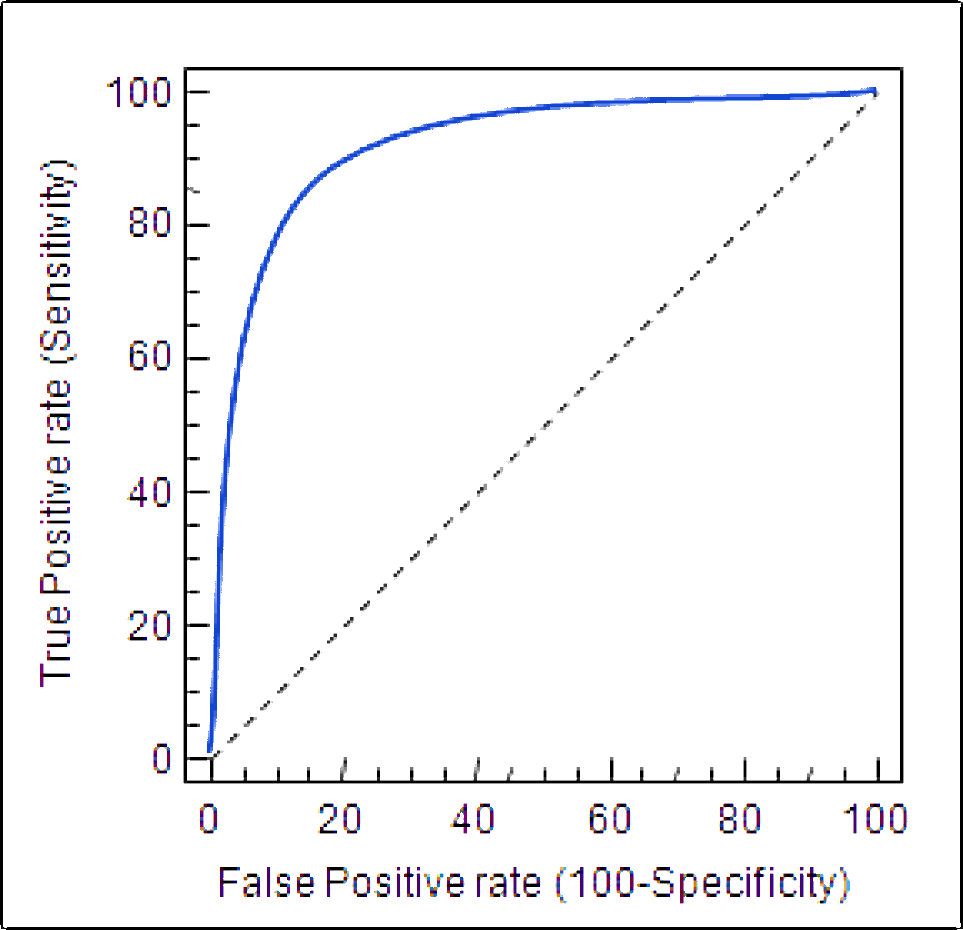
\includegraphics[scale=1]{Chapter2/Figures/roccurve2}
\end{center}
\caption[\ac{roc} curve]{\ac{roc} curve.}
\label{fig:roccurve}
\end{figure}



%%% Local Variables: 
%%% mode: latex
%%% TeX-master: "../thesis"
%%% End: 

\section{Conclusion}
This Chapter presented a broad-view of different aspects of machine learning and classification.
It also discusses, the most used and well-known techniques of each steps and the flow of the classification framework.
It is important to notice that the choice of different techniques in each step is application dependent and the best configuration is mostly found emprically.
Next chapters presents our proposed frameworks, where different techniques are employed in each step.

%%% Local Variables: 
%%% mode: latex
%%% TeX-master: "../thesis"
%%% End: 
